%% ====================================================================
%% Geometry-calibrated residual learning for spinal ligament landmarks
%% Medical Image Analysis (Elsevier) -- elsarticle, author-year citations
%%
%% Layout: the double-column 5p layout is permitted for LaTeX submissions
%% (MedIA Guide for Authors). For a single-column, double-spaced review copy,
%% swap the two \documentclass lines below.
%% Build: pdflatex -> bibtex -> pdflatex -> pdflatex  (Overleaf: default)
%% ====================================================================
\documentclass[5p,times,twocolumn,authoryear]{elsarticle}
%\documentclass[preprint,review,12pt,authoryear]{elsarticle}

\usepackage[T1]{fontenc}
\usepackage{newtxtext,newtxmath}
\usepackage{microtype}
\usepackage{graphicx}
\usepackage{xcolor}
\usepackage{booktabs}
\usepackage{multirow}
\usepackage{array}
\let\Bbbk\relax
\usepackage{amsmath,amssymb}
\usepackage{mathtools}
\usepackage{siunitx}
\usepackage[labelfont=bf,font=small,labelsep=period]{caption}
\usepackage{subcaption}
\usepackage{enumitem}
\usepackage{stfloats}
\usepackage{lineno}
\setcounter{topnumber}{5}
\setcounter{bottomnumber}{5}
\setcounter{totalnumber}{10}
\renewcommand{\topfraction}{0.95}
\renewcommand{\bottomfraction}{0.90}
\renewcommand{\textfraction}{0.05}
\renewcommand{\floatpagefraction}{0.85}
\renewcommand{\dbltopfraction}{0.95}
\renewcommand{\dblfloatpagefraction}{0.85}
\usepackage[colorlinks=true,linkcolor=black,citecolor=black,urlcolor=blue]{hyperref}

\graphicspath{{./figs/}}
\journal{Medical Image Analysis}

%% Revision marking. The clean and the highlighted versions are built from this one source:
%% \highlighttrue marks new or materially revised text, captions, and tables in blue;
%% \highlightfalse gives the clean version. Nothing else differs between the two.
\newif\ifhighlight
\highlightfalse
\definecolor{revcolor}{rgb}{0.0,0.27,0.68}
\newcommand{\rev}[1]{\ifhighlight{\color{revcolor}#1}\else#1\fi}
\newcommand{\revstart}{\ifhighlight\begingroup\color{revcolor}\fi}
\newcommand{\revend}{\ifhighlight\par\endgroup\fi}
\newcommand{\revfloat}{\ifhighlight\color{revcolor}\fi}
%% Rows of generated tables (paper/revision_tables.py); the primitive input keeps \bottomrule working.
\makeatletter\def\inputrows#1{\@@input #1 }\makeatother

% Line numbers help reviewers; comment out for the camera-ready version.
\linenumbers

\begin{document}
\begin{frontmatter}

\title{GCZ-RL: Geometry-Calibrated Residual Learning for Spinal Ligament Landmark Localization on Vertebral Surface Meshes}

%% ---------------------------------------------------------------------
%% AUTHORS -- to be confirmed by all authors before submission.
%% Dr. Maohua Lin is listed subject to his agreement and approval of the
%% manuscript, and remains the corresponding author as in the previous draft.
%% If this changes, move \corref{cor1} and \ead{} together.
%% ---------------------------------------------------------------------
\author[inst1]{Mohsen Ahmadi}
\author[inst2]{Maohua Lin\corref{cor1}}
\ead{mlin2014@fau.edu}
\author[inst1]{Yufei Tang}
\author[inst3]{Frank D. Vrionis}
\cortext[cor1]{Corresponding author.}
%% Full postal addresses are required on the title page (verify before submission).
\affiliation[inst1]{organization={Department of Electrical Engineering and Computer Science, Florida Atlantic University},
            addressline={777 Glades Road},
            city={Boca Raton},
            postcode={33431},
            state={FL},
            country={USA}}
\affiliation[inst2]{organization={Department of Biomedical Engineering, Florida Atlantic University},
            addressline={777 Glades Road},
            city={Boca Raton},
            postcode={33431},
            state={FL},
            country={USA}}
\affiliation[inst3]{organization={Department of Neurosurgery, Marcus Neuroscience Institute, Boca Raton Regional Hospital},
            city={Boca Raton},
            postcode={33486},
            state={FL},
            country={USA}}

\begin{abstract}
Spinal ligament attachment landmarks are needed for subject-specific spine models, but ligaments are invisible on computed tomography, so attachment sites must be placed on vertebral surface meshes. We present GCZ-RL, a geometry-calibrated residual-learning method for sparse ligament landmark localization from small annotated datasets. Geometry-calibrated zoning (GCZ) estimates ligament-specific admissible regions from annotations in normalized vertebral coordinates, rigidly aligns an annotated atlas vertebra to the target, and snaps transferred landmarks to target-mesh vertices inside these regions. An Extra Trees regressor then predicts each landmark's residual displacement. \rev{The predicted displacement is magnitude-bounded and projected onto the ligament-specific admissible surface region, with an anatomical side-preserving fallback for bilateral landmarks when required. All final predictions remain on the target vertebral surface.} The dataset comprises 57 annotated vertebrae of five subjects and seven ligament classes. The primary evaluation is leave-one-subject-out on all 14 lumbar vertebrae of three subjects, with calibration and model selection nested within the training subjects and a data-leakage test. GCZ-RL reduced the macro-averaged mean Euclidean error from 2.879 to 2.150~mm relative to GCZ (95\% bootstrap interval of the difference, $-1.08$ to $-0.38$~mm) and raised the share of landmarks within 5~mm from 86.0\% to 92.7\%, with improvement for each held-out subject. Segmentation-based landmark detection (SLD), run on the same vertebrae and scored identically, reached 2.224~mm and 90.4\%; the difference from GCZ-RL was not significant, and the two methods had complementary class-specific strengths. A vertebra-wise development analysis across cervical, thoracic, and lumbar levels showed the same direction of improvement.
\end{abstract}

\begin{keyword}
Spinal ligaments \sep Anatomical landmarks \sep Vertebral surface mesh \sep Atlas registration \sep Residual learning \sep Extra Trees \sep Patient-specific modeling
\end{keyword}

\end{frontmatter}

% =====================================================================
\section{Introduction}
\label{sec:introduction}

The passive stabilizing system of the spine is formed by several ligamentous structures that constrain intervertebral motion and contribute to load sharing, spinal stability, and facet joint mechanics~\citep{bogduk2012}. These structures include the anterior longitudinal ligament (ALL), posterior longitudinal ligament (PLL), ligamentum flavum (LF), interspinous ligament (ISL), supraspinous ligament (SSL), intertransverse ligament (ITL), and capsular ligament (CL). Their attachment sites define where ligaments are represented in subject-specific anatomical and computational models of the spine~\citep{ma2025posteriorligament,dreischarf2014,moramarco2010}. In current practice these sites are either placed manually, which is labor intensive, operator dependent, and difficult to scale, or derived from fixed geometric rules~\citep{ahmadi2025scirep,ahmadi2025worldneurosurgery,biswas2025sixligaments} that do not adapt to individual vertebral shape.

This paper addresses the underlying image-analysis problem: the localization of sparse ligament attachment landmarks on a vertebral surface mesh, evaluated against expert annotations. Downstream uses of the landmarks, such as finite element modeling, motivate the problem but are outside the scope of the present evaluation.

\revstart
This problem differs from generic vertebral landmark detection. Generic tasks, such as the vertebra labelling of the VerSe benchmark~\citep{sekuboyina2021}, locate a few salient points per vertebra, for example vertebral centroids, that are defined on the image and supported by hundreds of annotated scans. Ligament attachment sites are defined anatomically on the bone surface and differ between ligament classes in extent and shape, from the single annotated SSL point to the extended capsular footprints of CL. GCZ-RL is designed for this specialized localization problem, for which only small annotated datasets exist, rather than for generic landmark detection.
\revend

Spine image analysis has made strong progress in vertebral segmentation and surface extraction. Vertebral masks can be generated from CT or MRI using vertebra-specific segmentation strategies~\citep{lessmann2019}, self-configuring deep learning frameworks~\citep{isensee2021}, and public benchmarks such as VerSe~\citep{sekuboyina2021}. Large-scale segmentation tools have expanded automated anatomical extraction across many CT structures~\citep{wasserthal2023}, foundation-model approaches have increased the generality of medical image segmentation~\citep{ma2024medsam}, and large spine-specific datasets and 3D localization--segmentation models have improved the scalability of vertebral analysis~\citep{deng2025ctspine1k,lei2025medlsam}. A vertebral mask can be converted into a triangulated surface mesh by marching cubes~\citep{lorensen1987}. This surface captures patient-specific vertebral morphology, but it does not specify where ligament footprints or origin and insertion landmarks lie. A major step therefore remains between vertebral segmentation and a complete patient-specific spine model.

This gap matters because spine analysis is moving toward automated, geometry-aware, high-throughput modeling. Reviews of lumbar spine segmentation emphasize that external validation and dataset availability remain limitations~\citep{mendes2026lumbarreview}; boundary-sensitive segmentation highlights the importance of preserving vertebral morphology for downstream measurement~\citep{ji2026bsnet}; and open spine-analysis tools connect segmentation outputs with clinically meaningful geometric measurements~\citep{kowlagi2026olsia}. In parallel, surface-based registration has become important for transferring anatomical information across bones~\citep{wu2025neuralbonereg}. Ligament attachment placement, however, remains less standardized than vertebral segmentation: many workflows still depend on simplified geometric assumptions, manually selected landmarks, or template rules that do not adapt to specimen-specific shape.

Supervision for this task is scarce. Ligaments are not visible on CT, so attachment sites must be annotated by experts on three-dimensional vertebral surfaces, and datasets contain tens of vertebrae rather than thousands\rev{~\citep{kramer2024,blomenkamp2026sld}}. A network with enough capacity to learn vertebral shape, pose, and local attachment detail from so few examples is prone to overfitting, and an unconstrained regressor can place a landmark in the spinal canal or off the bone surface, which is anatomically implausible regardless of its numerical error. GCZ-RL addresses both problems by letting explicit anatomical constraints carry most of the localization and restricting learning to a constrained correction. Calibrated zoning learns where on the normalized surface each ligament class may appear; rigid registration transfers an expert landmark pattern from an atlas vertebra; and a residual regressor learns the systematic offset that rigid transfer leaves, with the corrected point projected back onto the admissible region.

GCZ-RL is designed around a simple principle: geometric anatomy should define the permissible solution space, while data-driven prediction should address only the residual localization error remaining after atlas transfer. This separation is particularly relevant when expert annotations are limited. Rather than learning unrestricted landmark coordinates, the method learns ligament-dependent search regions, initializes landmarks through rigid surface alignment, and refines their locations with bounded corrections that remain constrained to the target mesh. Its contribution is the integration of annotation-calibrated search spaces with fold-aware atlas transfer and constrained residual learning, evaluated against a registration-based geometric baseline and a dedicated ligament landmark detector. Specifically:
\begin{enumerate}[leftmargin=2em,itemsep=2pt,topsep=2pt]
  \item \textit{Calibrated anatomical constraints.} Ligament-specific admissible regions are estimated from annotations in a normalized vertebral coordinate space and act as constraints at every stage: \rev{the atlas-transferred landmark is selected inside them, the corrected landmark is projected onto them, and, for bilateral lateral classes, a side-preserving rule keeps each landmark on its side of the vertebra.}
  \item \textit{Constrained residual learning.} The learned component predicts only the residual between the constraint-satisfying geometric estimate and the expert landmark. Its correction is capped in magnitude by the spread of training residuals, can be switched off per class when validation does not support it, and is projected back onto the admissible region. Learning therefore refines a geometrically valid estimate: \rev{every corrected landmark is projected into the admissible region of its class, a bilateral landmark whose region has no vertex on its side keeps its geometric estimate, and every final prediction lies on the target vertebral surface.}
  \item \textit{Subject-level evaluation with a common evaluator.} The method is evaluated by leave-one-subject-out on the lumbar vertebrae, with the model and parameter selection of every fold nested inside its training subjects and a data-leakage test, and is compared with the SLD method~\citep{blomenkamp2026sld} on the same vertebrae with the same evaluator and with paired statistics. \rev{Each component is also examined on its own: the coverage and compactness of the candidate regions, a stage-wise ablation of the correction, the agreement and feature importance of the learned residuals, and the sensitivity of the atlas selection.} A vertebra-wise analysis on 57 vertebrae is reported as supplementary development evidence. Code, derived data, and trained models are released~\citep{gczrl2026code}.
\end{enumerate}

\section{Related work}
\label{sec:related}

Automated ligament landmark localization has been studied using atlas registration, point-cloud landmark transfer, geometric detection, and segmentation-based landmark prediction. \citet{aldhamari2019} proposed automatic detection of cervical spine ligament origin and insertion points using atlas-based registration. Such approaches can be effective when the reference and target anatomy are similar, but they are sensitive to registration error and local morphological variation. Generic point-cloud landmarking frameworks such as ALPACA~\citep{porto2021} transfer landmarks across three-dimensional biological structures using alignment and correspondence. They do not require training sets, but their generic nature does not encode spinal ligament-specific anatomical constraints.

\citet{kramer2024} detected spinal ligament landmarks on vertebral meshes using registration and 3D edge detection. More recently, \citet{blomenkamp2026sld} introduced segmentation-based landmark detection (SLD), which first segments the vertebral surface into anatomical regions by shape and then applies ligament-specific rules to locate attachment points; they reported a mean closest-point error of 0.7~mm on their annotated vertebrae and released both the implementation~\citep{spinetoolkit2026} and the annotations. SLD is a dedicated, rule-based landmark detector with no trainable parameters. GCZ-RL differs in that it calibrates its anatomical regions from annotations and learns a correction from data, which allows it to adapt to an annotation protocol and to classes whose attachment is not marked by a distinctive surface feature.

Registration-only approaches can produce anatomically implausible local correspondences when landmarks lie on curved rims, bilateral structures, or facet-related regions, and purely learned approaches typically require training sets larger than those available for ligament anatomy. GCZ-RL addresses both by learning admissible regions and a bounded correction from a small calibration set \rev{and by projecting every corrected prediction onto the admissible region of its class, so that all predictions remain on the vertebral surface}.

\section{Materials and methods}
\label{sec:methods}

\subsection{Dataset and study design}
\label{ssec:dataset}

The dataset consisted of 57 vertebrae from five subjects, each represented by a triangulated surface mesh with expert ligament attachment annotations. Forty-seven cervical, thoracic, and lumbar vertebrae of three subjects (S01--S03) come from VerSe CT data~\citep{sekuboyina2021}, and ten cervical vertebrae (C3--C7) of two further subjects (S04, S05) come from the public cervical ligament dataset that accompanies the SLD method~\citep{blomenkamp2026sld}, which is based on the cervical cases of \citet{aldhamari2019}. The expert annotations of all five subjects are those of the public ligament-landmark datasets released with SLD.

\revstart
\emph{Provenance of the reference annotations.} The attachment annotations were placed on the vertebral surface models rather than on CT images. The SLD publication describes them as manual annotations derived from anatomical knowledge and the literature, acquired in collaboration with medical professionals, and validated by medical experts~\citep{blomenkamp2026sld}; an earlier publication of the same group describes the manual annotation of randomly selected VerSe vertebral models by experts in the field~\citep{kramer2024}. Neither publication reports the number or qualifications of the annotators, the review procedure, or an inter- or intra-observer reliability analysis, and the data were not re-annotated for this study. The same released annotations serve as the reference for GCZ, GCZ-RL, and the evaluated SLD implementation, so that all methods are compared against a common anatomical reference under the same scoring protocol. Annotation variability is therefore contained in the reported errors of all three methods and cannot be separated from method error with the present data. These surface-based references define the localization target; the method does not require the ligaments to be visible in CT.
\revend

Seven ligament classes were considered: ALL, PLL, LF, ISL, SSL, ITL, and CL. The annotations are dense point sets along each attachment footprint (for example, a median of 23 ALL and 53 CL points per lumbar vertebra), except SSL (one point) and ITL (one point per side). \rev{Each class is stored as separate surface point sets for its parts (inferior and superior for ALL, PLL, LF, and ISL; left and right for ITL; four superior/inferior and left/right quadrants for CL), so the dense classes sample an attachment footprint rather than a single anatomical point, and the task addressed here is the localization of a sparse set of representative landmarks on each footprint.} Not every class is annotated at every level; SSL and ITL in particular are absent at some vertebrae.

Two analyses were performed (Table~\ref{tab:dataset}). The \emph{primary evaluation} is a patient-level leave-one-subject-out (LOSO) protocol on all lumbar vertebrae of the dataset (Section~\ref{ssec:loso}), in which model calibration and hyperparameter selection of each outer fold use only the vertebrae of the other two subjects. One methodological refinement, the side constraint for the lateral classes, was introduced after an earlier outer-fold result had been inspected (Section~\ref{ssec:loso}); the primary protocol therefore includes one post hoc design decision. The \emph{supplementary development analysis} uses a fixed vertebra-wise split into 20 calibration vertebrae (S01 L1--L5 and S02 C3--T10) and 37 held-out vertebrae (S02 T11--L4, S03 C3--L5, S04 and S05 C3--C7). Quantitative scores are computed on the 27 held-out VerSe vertebrae; the ten held-out cervical vertebrae of S04 and S05 are predicted but were not scored. Because this split is made at the vertebral level, S02 contributes vertebrae to both partitions, and development outputs informed the per-class model configuration (Section~\ref{ssec:gcz_rl}). Its results are therefore reported as descriptive development evidence across cervical, thoracic, and lumbar levels, not as an independent assessment of generalization. The two analyses have different roles and are not pooled.

\begin{table*}[!t]
\centering
\caption{Dataset organization and evaluation use. The primary evaluation consists of 14 lumbar vertebrae from three subjects under patient-level LOSO\rev{; the number of independent units is three subjects, and vertebrae, vertebra--class cases, and landmarks are nested within them}. The supplementary development analysis uses 20 calibration and 37 held-out vertebrae; all held-out vertebrae receive predictions, the VerSe subset is scored quantitatively, and the ten S04--S05 cervical vertebrae receive predictions only. The two analyses are not pooled.}
\label{tab:dataset}
\renewcommand{\arraystretch}{1.12}
\small
\begin{tabular}{@{}p{0.27\textwidth}cp{0.56\textwidth}@{}}
\toprule
\textbf{Subset / item} & \textbf{No.} & \textbf{Use} \\
\midrule
Annotated vertebrae & 57 & Five subjects: S01--S03 from VerSe (47 vertebrae), S04--S05 from the SLD cervical dataset (10 vertebrae). \\
Patient-level cohort (primary, LOSO) & 14 & Lumbar vertebrae of three subjects (S01 L1--L5, S02 L1--L4, S03 L1--L5); three folds, each holding out one subject. \\
\rev{Independent subjects (primary)} & \rev{3} & \rev{Unit of the outer cross-validation; every learned quantity of a fold comes from the two training subjects.} \\
\rev{Vertebra--class cases (primary)} & \rev{98} & \rev{14 vertebrae $\times$ 7 classes; unit of the paired Wilcoxon tests. The bootstrap resamples the 14 vertebrae.} \\
\rev{Reference points (primary)} & \rev{2165} & \rev{Expert points of the 98 cases; GCZ and GCZ-RL predict 742 landmarks each, SLD 938 (Supplementary Table~S2).} \\
Calibration vertebrae (development) & 20 & Threshold estimation, atlas, residual-regressor training, correction bounds, and regressor comparison. \\
Held-out vertebrae (development) & 37 & Held-out prediction; quantitative evaluation on the 27 held-out VerSe vertebrae. \\
Ligament classes & 7 & ALL, PLL, LF, ISL, SSL, ITL, and CL. \\
Evaluation protocol & -- & Same annotations, ligament grouping, one-to-one matching, Euclidean error, and averaging for all methods. \\
\bottomrule
\end{tabular}
\end{table*}

\subsection{Overview of the GCZ-RL pipeline}
\label{ssec:pipeline}

Figure~\ref{fig:gcz_landmark_pipeline} summarizes the pipeline. The calibration component learns ligament-specific admissible regions and assembles the annotated atlas. The prediction component aligns the atlas to each target vertebra by ICP and selects GCZ landmarks only inside the admissible regions. The residual-learning component predicts a bounded correction for each GCZ landmark with Extra Trees and projects the corrected point back onto the admissible region. The output is a sparse set of at most ten ligament attachment landmarks per class, each a vertex of the target mesh.

\revstart
The three stages have complementary roles, and each is evaluated separately in Section~\ref{ssec:component_results}. Anatomy-informed candidate-region calibration (GCZ zoning) learns class-specific admissible search regions rather than exact anatomical point correspondences; atlas-based geometric initialization by rigid ICP supplies a global pose estimate rather than a guarantee of local correspondence; and constrained residual refinement adjusts that initialization using geometry-derived information while retaining the admissible surface constraints.
\revend

\begin{figure*}[!t]
\centering
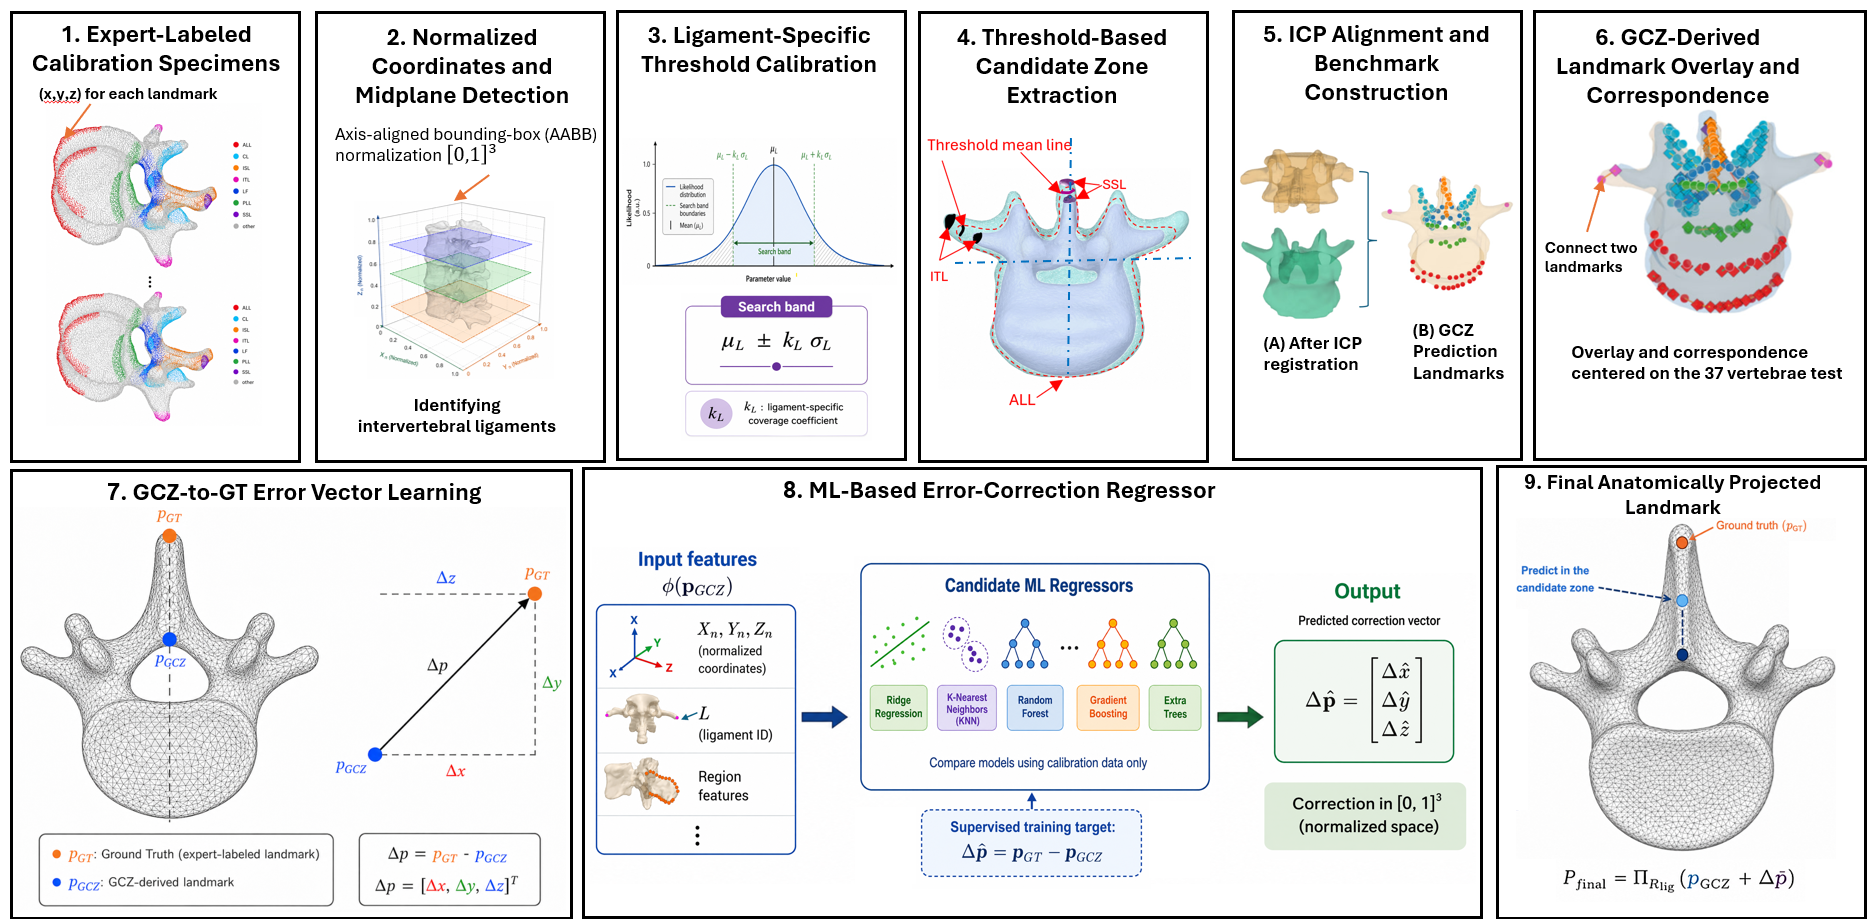
\includegraphics[width=1.0\textwidth]{fig_gcz_pipeline_benchmark_style4.png}
\caption{GCZ-RL landmark reconstruction workflow. The calibration branch uses annotated calibration vertebrae to define normalized anatomical coordinates, calibrate ligament-specific threshold bands, construct candidate regions, and assemble the annotated atlas. The prediction branch applies the learned thresholds to each target vertebra, aligns the atlas by ICP, and selects initial GCZ landmarks inside the candidate regions. The residual-learning branch computes GCZ-to-expert correction vectors on training data only, trains the Extra Trees regressor, adds the bounded predicted correction to each GCZ point, and projects the corrected point back onto the candidate region before evaluation. \rev{The same steps on real data of a held-out vertebra are shown in Supplementary Fig.~S4.}}
\label{fig:gcz_landmark_pipeline}
\end{figure*}

\subsection{Surface normalization and midplane references}
\label{ssec:preprocess}

Each vertebral surface mesh, in the LPS frame of the source CT, was mapped into a normalized coordinate frame by axis-aligned bounding-box (AABB) normalization:
\begin{equation}
  x_n = \frac{x-x_{\min}}{x_{\max}-x_{\min}}, \quad
  y_n = \frac{y-y_{\min}}{y_{\max}-y_{\min}}, \quad
  z_n = \frac{z-z_{\min}}{z_{\max}-z_{\min}} .
  \label{eq:aabb}
\end{equation}
After normalization, all surface vertices lie in a common $[0,1]^3$ domain. This domain is used to learn thresholds and search regions, while landmark errors are computed in millimeters in the original frame. \rev{The normalization supports the calibration of search regions; it does not establish point-to-point anatomical correspondence between vertebrae, which is left to the atlas transfer and the residual correction.}

For lumbar levels, intervertebral midplanes were used as references for separating superior and inferior regions. For adjacent vertebrae $V_k$ and $V_{k+1}$, the midplane position was
\begin{equation}
Z_{\mathrm{mp}}(V_k,V_{k+1}) = \frac{Z_{\mathrm{cen}}(V_k)+Z_{\mathrm{cen}}(V_{k+1})}{2},
\label{eq:midplane}
\end{equation}
where $Z_{\mathrm{cen}}$ is the normalized centroid coordinate along the inferior--superior axis. For two subjects of visibly different size, the normalized midplane positions agreed to within 0.03 at every lumbar level (0.24 and 0.21 at L5--L4, 0.42 and 0.40 at L4--L3, 0.60 and 0.60 at L3--L2, 0.78 and 0.79 at L2--L1; Fig.~\ref{fig:preprocess_montage}D).

\begin{figure*}[!t]
\centering
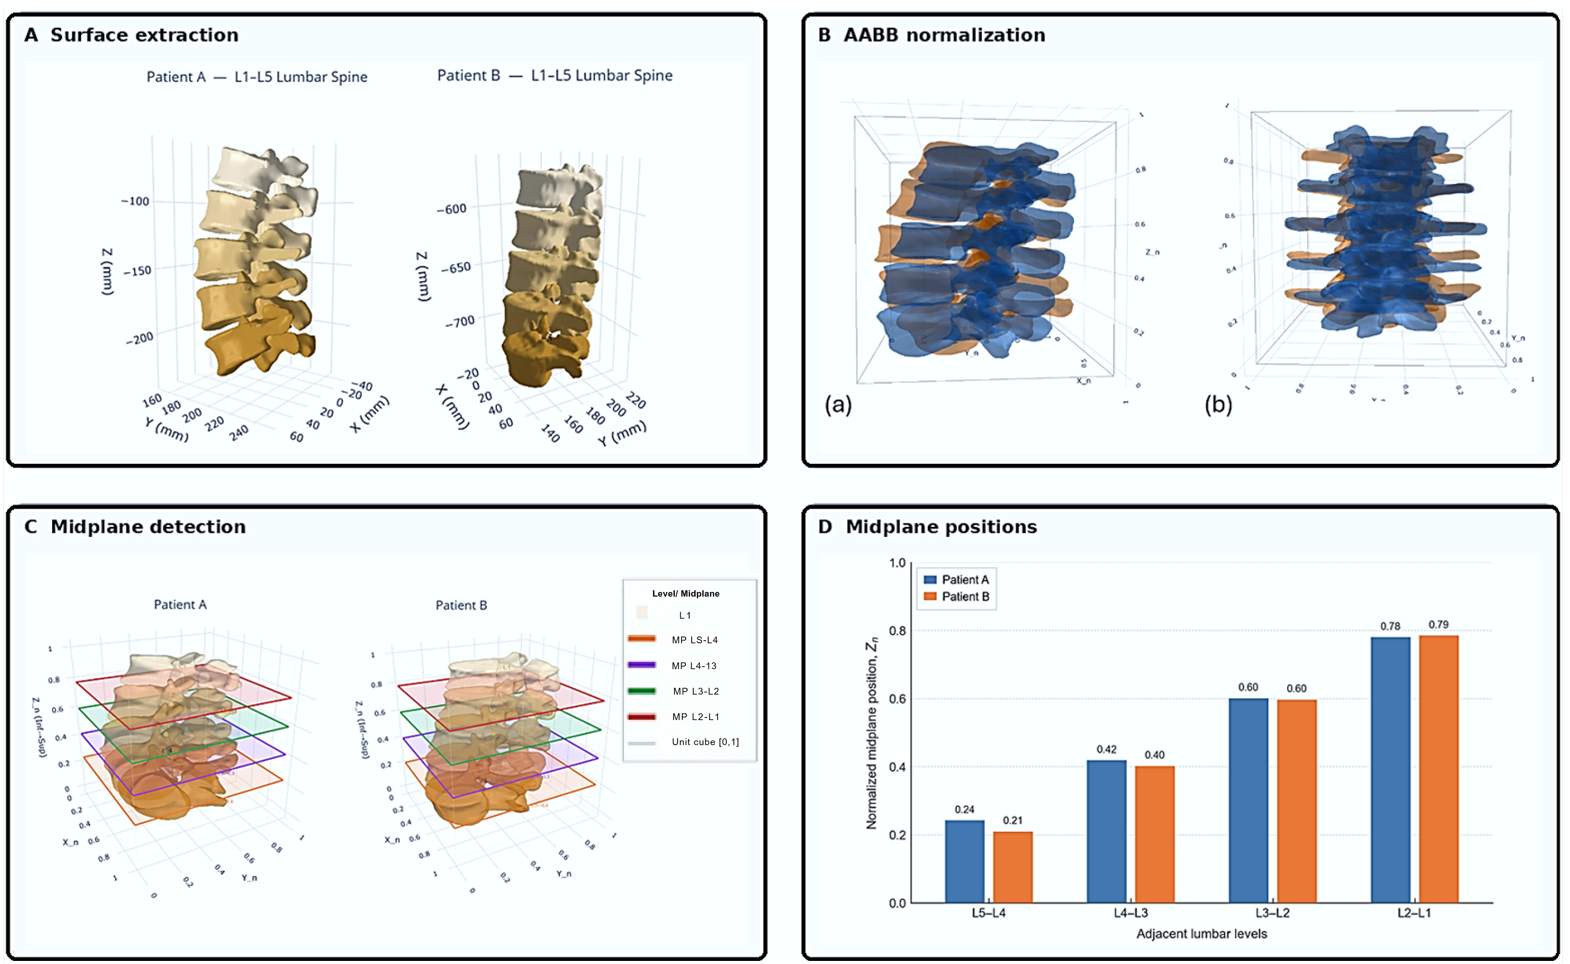
\includegraphics[width=0.99\textwidth]{fig_preprocessing_montage.png}
\caption{Preprocessing and normalized anatomical reference construction. (A) Vertebral surface meshes of two subjects of different size. (B) AABB normalization places surfaces in a shared $[0,1]^3$ coordinate space. (C) Midplanes provide level-wise anatomical references. (D) Normalized midplane positions agree closely between the two subjects at every lumbar level.}
\label{fig:preprocess_montage}
\end{figure*}

\subsection{Threshold calibration and candidate-region assignment}
\label{ssec:thresholds}

For each ligament class $L$, the expert annotations of the training vertebrae were mapped into the normalized domain of their own vertebra. The relevant normalized coordinate for that class is denoted $d_L(\mathbf{v})$. Pooling the training values gives a mean $\mu_L$ and sample standard deviation $\sigma_L$, which define a ligament-specific search band
\begin{equation}
  T_L^- = \mu_L - k_L\sigma_L, \qquad
  T_L^+ = \mu_L + k_L\sigma_L ,
  \label{eq:threshold_band}
\end{equation}
where $k_L$ is a coverage coefficient ($k_L=2$ for all classes) and the band is clipped to $[0,1]$. In the implementation, $d_L$ comprises three normalized quantities, $y_n$, $|x_n-0.5|$, and $z_n$, each with its own band, and the candidate region $\mathcal{R}_L$ is the set of surface vertices that lie inside all three bands,
\begin{equation}
  \mathcal{R}_L = \{\mathbf{v} : T_L^- \le d_L(\mathbf{v}) \le T_L^+ \ \text{for each of the three quantities}\}.
  \label{eq:threshold_rule}
\end{equation}
If fewer than 64 vertices remain, the $z_n$ band is dropped (Supplementary Section~S2). The threshold does not predict the final landmark; it defines where the algorithm may search. ALL is searched in an anterior region, PLL in a posterior, canal-side region, CL near the articular processes, and so on, and bilateral classes retain separate left and right patches. In the patient-level cohort, whose meshes have a median of 33{,}445 vertices, the regions of the larger classes retain several thousand vertices and those of SSL and ITL far fewer.

The calibrated regions define ligament-specific geometric search spaces on the target surface rather than independent segmentations of the attachment footprints. Their role is to exclude implausible candidates and provide a reproducible constraint for initial transfer and subsequent residual projection. All class-specific bands and the stated fallback rule are derived from the corresponding training partition. Across held-out vertebrae of the patient-level folds, 90.0\% of reference landmarks were contained in their class-specific candidate regions (range across classes: 83.7\% for PLL to 96.7\% for ALL; Supplementary Table~S4). This containment rate is an upper bound on how close GCZ-RL can come to the reference points that fall outside the region of their class. \rev{Containment alone would be uninformative if the regions admitted most of the surface. Measured by triangle area, the regions used for projection cover a median of 0.1\% (ITL) to 26.9\% (CL) of the vertebral surface (Table~\ref{tab:compactness}), so they contain most reference landmarks while excluding most of the vertebra.}

\begin{figure*}[!t]
\centering
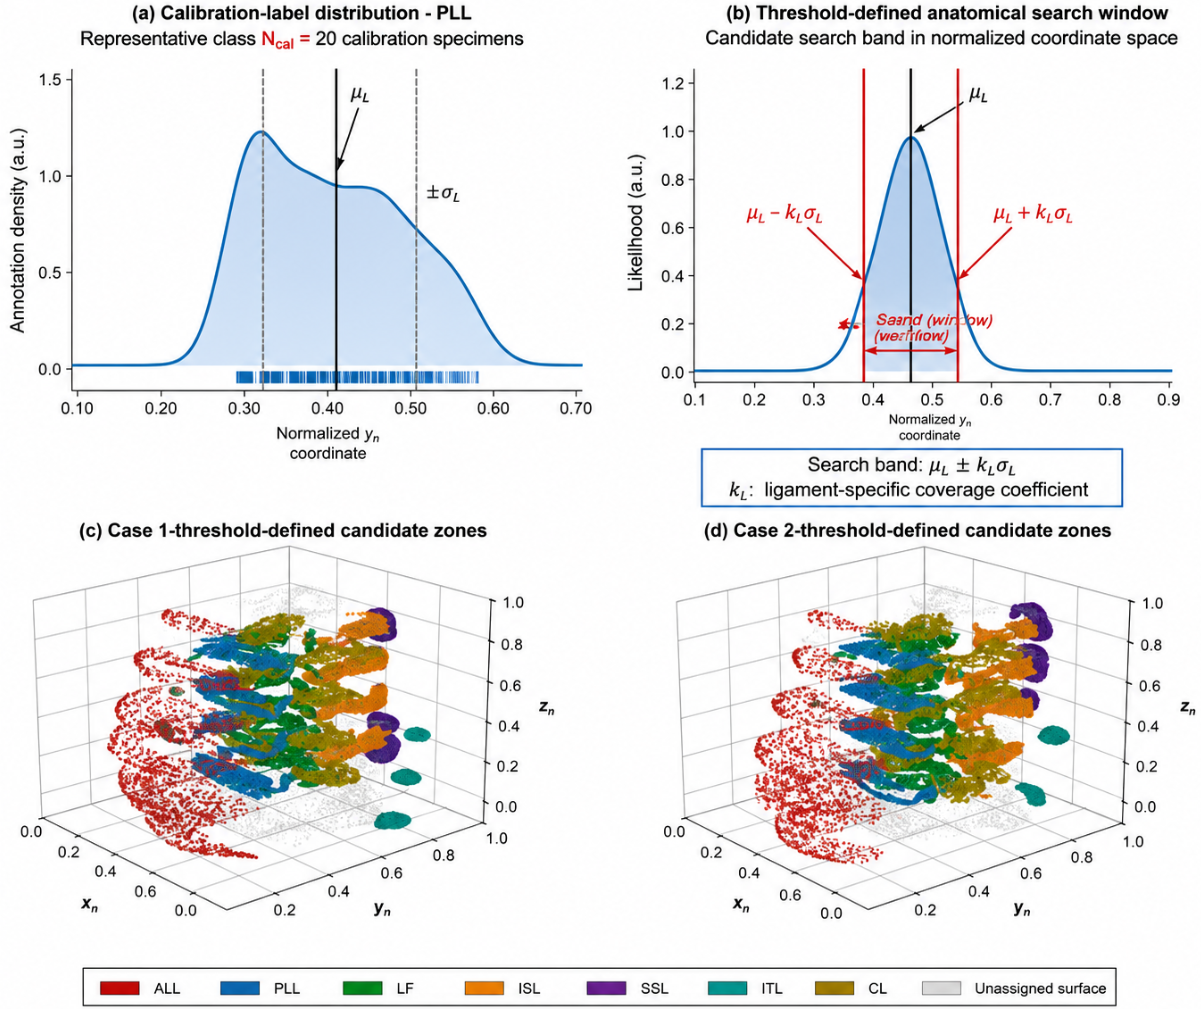
\includegraphics[width=0.80\textwidth]{fig_threshold_candidate_combined1.png}
\caption{Threshold calibration and GCZ candidate regions. The calibration annotations define a mean location and variability for each ligament-specific search quantity. The band $\mu_L \pm k_L\sigma_L$ defines the admissible candidate region. The resulting zones are search regions, not the final landmarks and not attachment footprints\rev{; Fig.~\ref{fig:regions_footprints} shows the real regions of a held-out vertebra next to its expert annotations}.}
\label{fig:threshold_candidate}
\end{figure*}

\subsection{Atlas transfer by iterative closest point}
\label{ssec:atlas}

The atlas is formed separately for each training partition. In each patient-level fold it consists of all annotated lumbar vertebrae of the two training subjects, and no mesh or landmark of the held-out subject is used to select or align it; when the training vertebrae of one subject are themselves predicted to generate residual targets, the atlas consists of the vertebrae of the other training subject. In the development analysis the atlas consists of the five annotated lumbar vertebrae (L1--L5) of one calibration subject; because the held-out vertebrae of that analysis include cervical and thoracic levels, its atlas transfer is in part a cross-level transfer, and its results should not be read as evidence of equal reliability across spinal regions. Each atlas vertebra is rigidly aligned to the target vertebra by iterative closest point (ICP) registration~\citep{besl1992,chen1992}, which alternates nearest-neighbor correspondence with the closed-form least-squares rigid fit~\citep{umeyama1991}:
\begin{equation}
  (\mathbf{R}^*,\mathbf{t}^*) =
  \arg\min_{\mathbf{R}\in SO(3),\mathbf{t}}
  \sum_j \left\|\mathbf{R}\mathbf{p}_j+\mathbf{t}-
  \mathrm{NN}(\mathbf{R}\mathbf{p}_j+\mathbf{t};\mathcal{Q})\right\|_2^2 ,
  \label{eq:icp}
\end{equation}
where $\mathbf{p}_j$ are points of the atlas surface, $\mathcal{Q}$ is the target surface, and $\mathrm{NN}(\cdot;\mathcal{Q})$ is the nearest target point. Atlas selection uses a short ICP for every atlas vertebra (1200 randomly sampled atlas points, at most 40 iterations); the atlas vertebra with the lowest mean nearest-neighbor residual is retained, whatever its vertebral level, and is aligned again with a longer ICP (5000 sampled points, at most 150 iterations). Its expert landmarks are transferred to the target with the same transformation, $\mathbf{p}^{\mathrm{tr}}_L = \mathbf{R}^{*}\mathbf{p}^{\mathrm{ref}}_L + \mathbf{t}^{*}$. ICP estimates six parameters, so the transfer carries pose but not shape; the shape-dependent remainder is left to the residual stage. \rev{ICP thus serves as a geometric initialization. Atlas selection optimizes surface alignment rather than anatomical correspondence, and a lower ICP residual does not guarantee a better landmark transfer; the relation between the two is examined in Section~\ref{ssec:component_results}.}

\subsection{GCZ landmark selection}
\label{ssec:prediction}

For each target vertebra, the learned thresholds are applied to obtain the candidate regions, and each transferred landmark is replaced by the closest vertex of the target mesh inside the region of its class,
\begin{equation}
  \mathbf{p}_{\mathrm{GCZ}} = \operatorname*{argmin}_{\mathbf{v}\in\mathcal{R}_L} \left\| \mathbf{v} - \mathbf{p}^{\mathrm{tr}}_L \right\|_2 .
  \label{eq:gcz_select}
\end{equation}
Transferred landmarks farther than 15~mm from the region are discarded when enough nearer ones remain. For LF and ITL the snapping is performed separately for the left and right halves of the vertebra (split at the $x$-centroid of the mesh), and for CL separately for its four superior/inferior and left/right quadrants. Duplicate vertices are merged, and if more than ten distinct vertices remain, ten are retained by farthest-point sampling. The result is a set of at most ten surface vertices per class (one for SSL and two for ITL, the number of atlas annotations of these classes), each inside the admissible region of its class. This geometry-only prediction is referred to as the original GCZ configuration.

\begin{figure*}[!t]
\centering
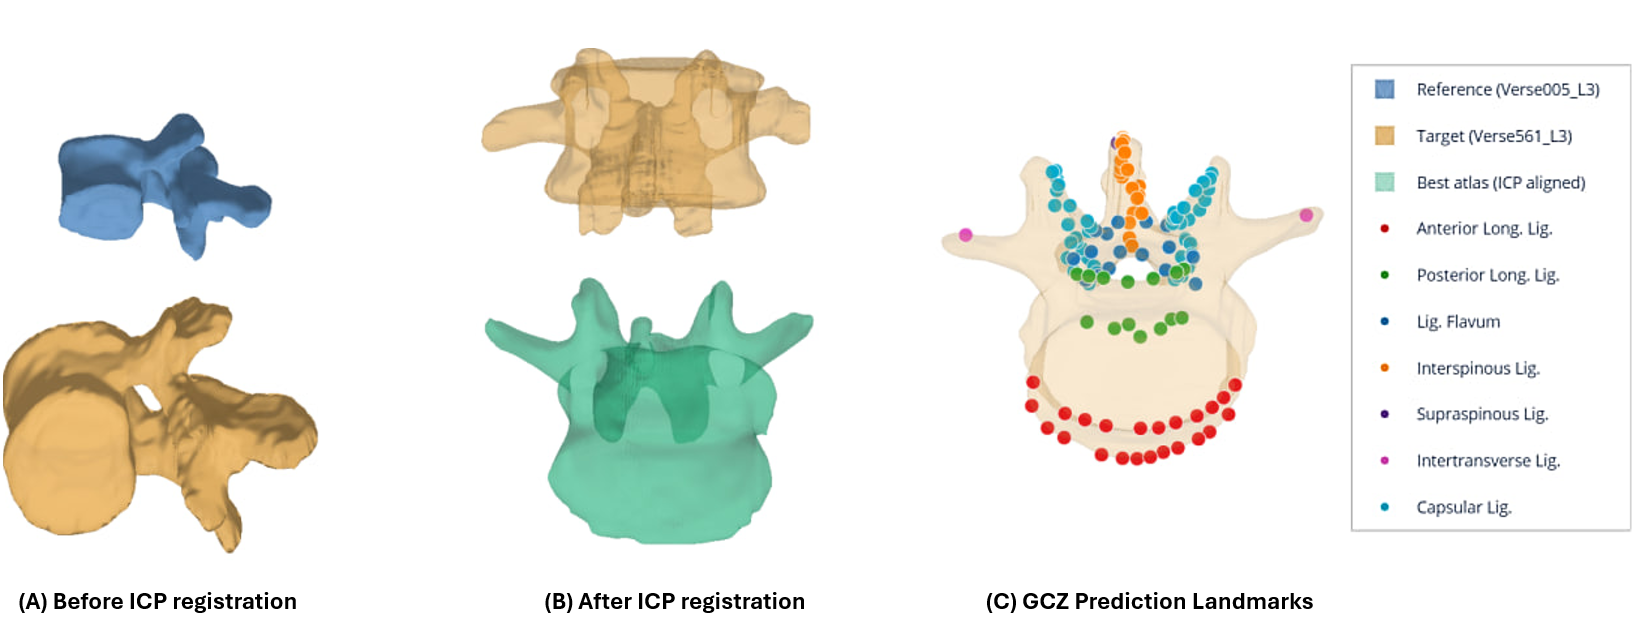
\includegraphics[width=0.98\textwidth]{fig_prediction_pipeline.png}
\caption{Representative atlas-to-target prediction workflow. An annotated atlas vertebra is aligned to a held-out vertebra. After ICP alignment, ligament-specific regions constrain where GCZ landmarks can be selected. Errors are computed separately from paired landmark distances.}
\label{fig:prediction_pipeline}
\end{figure*}

\subsection{Bounded residual-learning correction}
\label{ssec:gcz_rl}

Rigid transfer leaves a displacement between the GCZ point and the expert landmark that is systematic for a given ligament class, because six rigid parameters cannot follow differences in the length of a spinous process or the breadth of a lamina. GCZ-RL learns this displacement (Fig.~\ref{fig:gcz_residual_learning_framework}). On training vertebrae, the GCZ points of each class are paired one-to-one with expert landmarks by Hungarian assignment~\citep{kuhn1955}, and the residual target of a GCZ point is
\begin{equation}
  \Delta \mathbf{p}_{\mathrm{true}} = \mathbf{p}_{\mathrm{GT}} - \mathbf{p}_{\mathrm{GCZ}} .
  \label{eq:residual_target}
\end{equation}
Each training GCZ point is obtained with an atlas that excludes its own vertebra, as for an unseen vertebra. A 36-dimensional feature vector $\boldsymbol{\phi}_{\mathrm{GCZ}}$ describes the GCZ point: its normalized coordinates, the ligament class, the vertebral level, descriptors of the candidate region and of the local surface, and its offset from the mean training landmark position of its class. Every feature is defined, with its formula and source, in Supplementary Table~S1. For LF, ISL, ITL, and CL, each sample is augmented by its mirror image about the sagittal plane through the vertex centroid, with the lateral component of the residual negated, giving 1683 training samples from the 20 calibration vertebrae of the development analysis. Samples of the same vertebra, and mirrored copies in particular, are correlated and are not independent specimens; every cross-validation split therefore groups all samples of a vertebra (development analysis) or of a subject (patient-level folds) on the same side, and only original, non-mirrored samples are used for validation. An Extra Trees regressor~\citep{geurts2006} $F_{\mathrm{ET}}$ predicts the correction,
\begin{equation}
  \Delta \hat{\mathbf{p}} = F_{\mathrm{ET}}(\boldsymbol{\phi}_{\mathrm{GCZ}}).
  \label{eq:residual_prediction}
\end{equation}
The correction is clipped to a ligament-specific bound $\tau_L$, the mean plus two standard deviations of the training residual magnitudes of class $L$, added to the GCZ point, and projected onto the candidate region,
\begin{equation}
  \tilde{\mathbf{p}} = \Pi_L\!\left(\mathbf{p}_{\mathrm{GCZ}} + \mathrm{clip}(\Delta \hat{\mathbf{p}}, \tau_L)\right),
  \qquad
  \Pi_L(\mathbf{x}) = \operatorname*{argmin}_{\mathbf{v}\in\mathcal{R}_L} \left\| \mathbf{v} - \mathbf{x} \right\|_2 ,
  \label{eq:corrected_point}
\end{equation}
where $\mathrm{clip}(\mathbf{a},\tau)=\mathbf{a}\,\min(1,\tau/\|\mathbf{a}\|_2)$ preserves the direction of the correction and caps its length. A ligament-specific blend weight $\alpha_L$ then scales the projected correction, and the result is projected again,
\begin{equation}
  \mathbf{p}_{\mathrm{final}} = \Pi_L\!\left(\mathbf{p}_{\mathrm{GCZ}} + \alpha_L\,(\tilde{\mathbf{p}} - \mathbf{p}_{\mathrm{GCZ}})\right).
  \label{eq:projection}
\end{equation}
With $\alpha_L=1$ the output is $\tilde{\mathbf{p}}$, and with $\alpha_L=0$ it is the GCZ point (which lies in $\mathcal{R}_L$ for every class and fold in which $\alpha_L=0$ was selected). Clipping bounds the damage that an extrapolating regressor can do, and projection makes the output a surface vertex of the admissible region $\mathcal{R}_L$\rev{; the one exception, introduced by the side constraint of Section~\ref{ssec:loso}, is a bilateral point whose region has no vertex on its side, which keeps its GCZ position, a surface vertex of the GCZ selection region}. Held-out annotations are not used for residual-model fitting, correction bounds, or projection.

\revstart
The elements of the correction have distinct roles. The residual prediction supplies the learned, shape-dependent displacement; clipping limits its length to the range observed in training; the blend weight $\alpha_L$, chosen by nested validation in the primary evaluation, scales the correction or switches it off for classes in which it does not help on the training subjects; projection returns the point to a vertex of the admissible region; and, in the primary evaluation, the side constraint of Section~\ref{ssec:loso} keeps each bilateral landmark on its side of the vertebra. All 36 features are computed from the target mesh, the GCZ point, and quantities learned from the training vertebrae, so all of them are available at inference. The contribution of each element is measured in Section~\ref{ssec:component_results}.
\revend

\begin{figure*}[!t]
\centering
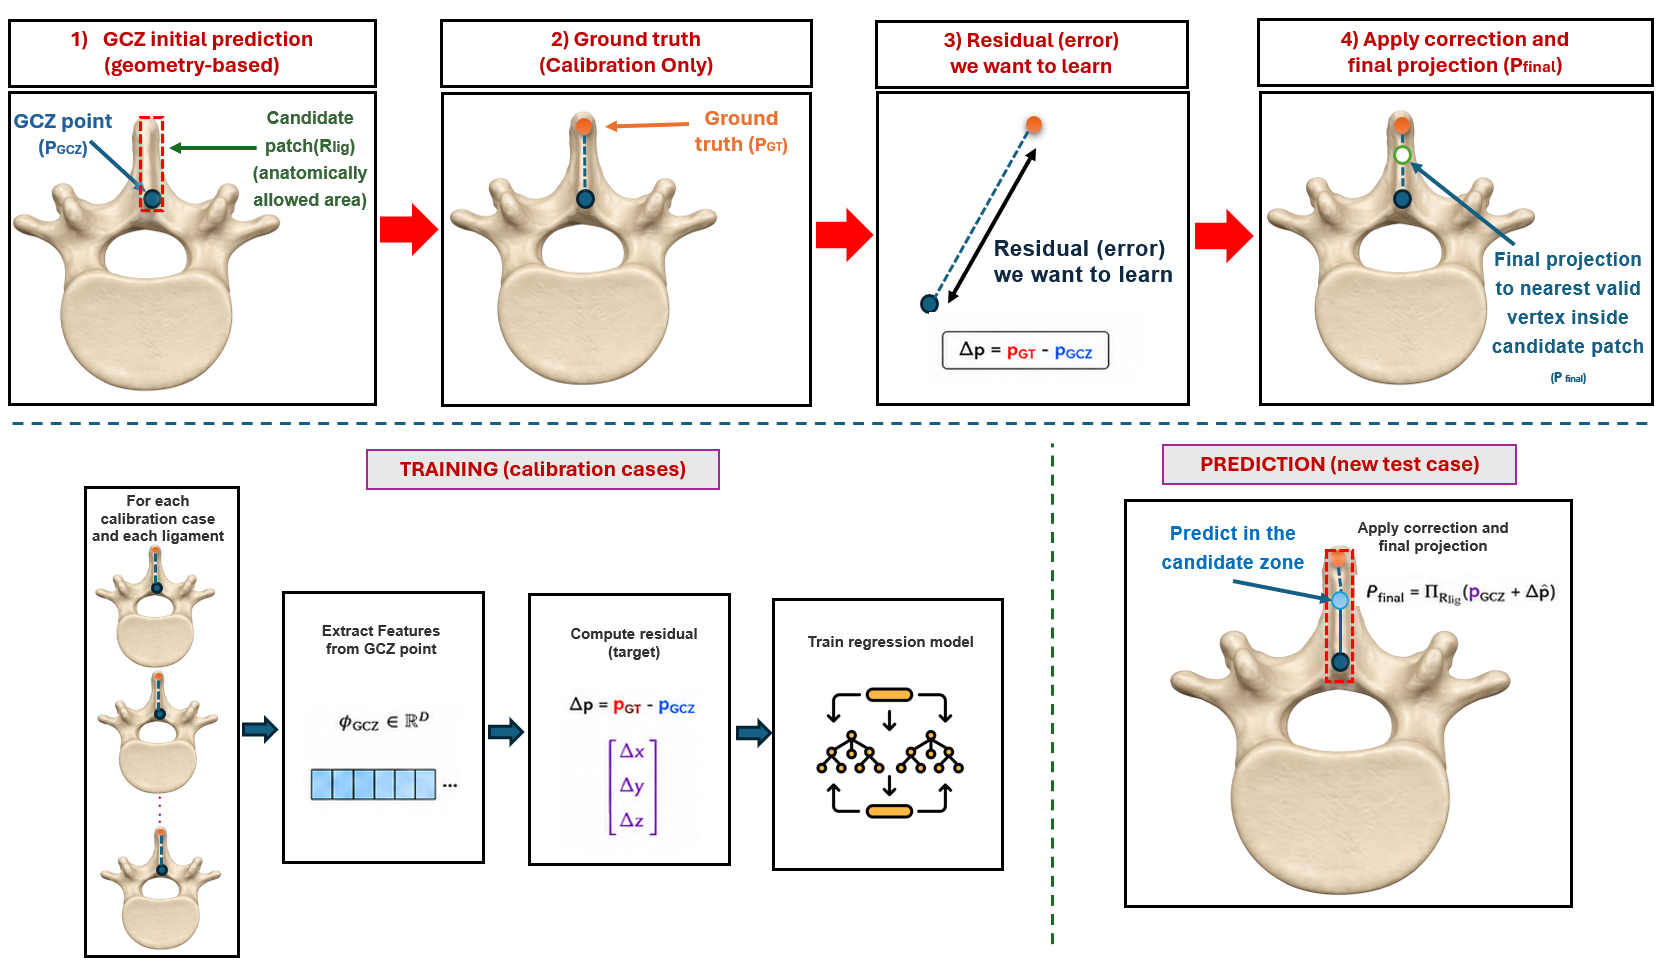
\includegraphics[width=0.99\textwidth,keepaspectratio]{gcz_residual_learning_framework.png}
\caption{Geometry-constrained GCZ-RL correction. Residuals between GCZ and expert landmarks on training data are used to compare residual regressors and to train the Extra Trees regressor. At inference, the bounded predicted correction is added to the GCZ point, which is then projected to the nearest admissible vertex of its ligament-specific region. \rev{The applied corrections on a held-out vertebra are shown in Supplementary Fig.~S5.}}
\label{fig:gcz_residual_learning_framework}
\end{figure*}

\paragraph{Regressor selection} Five residual regressors with different inductive biases were compared on the calibration vertebrae of the development analysis: ridge regression, $k$-nearest neighbors, random forests~\citep{breiman2001}, gradient boosting, and Extra Trees, all implemented in scikit-learn~\citep{pedregosa2011}. Each was evaluated by leave-one-vertebra-out over the 20 calibration vertebrae, with the blend weight $\alpha \in \{0.70, 0.85, 1.00, 1.10, 1.20\}$, and for each family the best of its configurations is reported (one configuration each for ridge regression, nearest neighbors, and random forests, two gradient-boosting implementations, and four Extra Trees configurations; Supplementary Table~S5). In each leave-one-vertebra-out fold the candidate regions, class prior, and correction bound used for features and projection were recomputed without the held-out vertebra; the GCZ inputs of the calibration vertebrae were computed once, with zones from all 20 calibration vertebrae. In the supplementary development analysis, the reported configuration was partly selected after held-out outputs had been examined: two complete Extra Trees runs that differed in their configurations were compared, and for each class the configuration of one of them was retained (one run for LF and SSL, the other for the remaining classes). These held-out results were therefore involved in model development and are not unbiased final-test estimates. The primary, patient-level analysis instead selects the regressor configuration and the blend weight separately within each outer fold, by an inner leave-one-subject-out procedure restricted to the two training subjects (Section~\ref{ssec:loso}), so that no held-out annotation is used for hyperparameter selection; the post hoc side constraint of Section~\ref{ssec:loso} is the one design decision not covered by this nesting.

\subsection{Correspondence and error metrics}
\label{ssec:correspondence}

Predicted and expert landmarks must be paired before an error can be computed. For all methods, the evaluation uses one-to-one Hungarian matching~\citep{kuhn1955} within each ligament class of each vertebra. For a matched predicted landmark $\hat{\mathbf{p}}_i$ and expert landmark $\mathbf{g}_{\pi(i)}$, the error is
\begin{equation}
  e_i = \left\|\hat{\mathbf{p}}_i - \mathbf{g}_{\pi(i)}\right\|_2 .
  \label{eq:error}
\end{equation}
The reported error, denoted MAE for consistency with prior landmark-localization work, is the mean Euclidean distance between matched predicted and reference landmarks, not the mean absolute error of individual coordinates. It is averaged over the matched pairs of each vertebra--class case, then over the vertebrae of each class, and finally over the seven classes (macro average). Pass@5 is the percentage of matched pairs with $e_i \le 5$~mm; in the vertebra-wise development analysis it pools the pairs of each class before averaging over classes, and in the patient-level evaluation it is averaged over vertebra--class cases. For GCZ and GCZ-RL, which predict the same number of landmarks for every vertebra of a class, the two conventions coincide; for SLD the pooled patient-level value is 90.2\% instead of 90.4\%.

The number of predicted landmarks per class need not equal the number of annotated reference points. One-to-one matching therefore pairs at most the smaller of the two sets, and any remaining points are unpaired. MAE and Pass@5 measure how close the paired landmarks lie to the annotated footprint; they do not penalize footprint regions without a prediction. To make this explicit, the numbers of reference, predicted, matched, and unpaired points are reported for every method, class, and subject (Supplementary Table~S2), together with matching-independent metrics (Supplementary Table~S3): the closest-point distance from each prediction to the reference set, which corresponds to the error reported by \citet{blomenkamp2026sld}; the closest-point distance from each reference point to the prediction set; their symmetric mean; and the percentage of all reference points whose nearest prediction lies within 5~mm. No method had a missing output for any vertebra--class case, so no case is dropped from the averages.

\revstart
These metrics answer different questions, and the main ones are reported side by side in Table~\ref{tab:overall}. Matched-pair MAE and Pass@5 ask how close each predicted landmark lies to a distinct reference point. The prediction-to-reference (P$\rightarrow$R) closest-point distance asks whether each prediction lies on the annotated footprint, without requiring distinct partners. The reference-to-prediction (R$\rightarrow$P) distance and the share of reference points within 5~mm of a prediction ask how much of the footprint the sparse predictions represent; their symmetric mean combines both directions. The share of reference points paired by Hungarian matching depends mainly on the number of predicted landmarks and is not a measure of geometric coverage. In every case of the primary evaluation the predicted set was the smaller one, so every prediction was paired, and the unpaired points are reference points.
\revend

\paragraph{Statistical analysis} Paired differences between methods were tested over the 98 vertebra--class cases of the primary evaluation with the two-sided Wilcoxon signed-rank test, and 95\% confidence intervals of the difference in macro-averaged MAE were obtained with a cluster bootstrap that resamples the 14 vertebrae with replacement (5000 replicates). Because cases are nested in vertebrae and vertebrae in only three subjects, these statistics describe the consistency of the paired differences within this cohort; they do not support population-level inference. \rev{Statements of statistical significance therefore refer to paired comparisons within the evaluated set, and the consistency of each effect across the three held-out subjects is reported with them.} \rev{The component analyses of Section~\ref{ssec:component_results} were defined after the primary results were known; they decompose the fixed, already evaluated pipeline and select nothing.}

\subsection{SLD comparator}
\label{ssec:sld_evaluation}

SLD~\citep{blomenkamp2026sld} was run on the same vertebrae and scored with the same evaluator. It has fixed parameters and uses no annotations. In the vertebra-wise development analysis, SLD was run through a standalone batch adaptation of the public SpineToolkit workflow; this run used a coarser surface remeshing than the published configuration and passed the meshes to the SLD code in their LPS frame, whereas the code assumes the RAS frame of 3D Slicer. These development results are not an appropriate basis for ranking the methods. For the primary patient-level comparison, SLD was evaluated with the released SpineToolkit implementation~\citep{spinetoolkit2026} and its published preprocessing (surface remeshing to 5000 clusters, smoothing, hole filling, and snapping of each landmark to the input mesh), including conversion of input meshes to the expected RAS coordinates and conversion of predicted landmarks back to the common evaluation frame. The centerline component, which normally uses the VMTK extension of 3D Slicer, was approximated with cross-section centroids because VMTK was not available in the batch environment; no SLD parameter was tuned. All three methods were evaluated against the same annotations and with the same pairing and aggregation rules. The numerical comparison therefore refers specifically to the SLD implementation evaluated here.

\subsection{Primary evaluation: patient-level leave-one-subject-out}
\label{ssec:loso}

The patient-level cohort consists of every lumbar vertebra of the dataset: S01 L1--L5, S02 L1--L4 (the scan ends at L4), and S03 L1--L5, that is, 14 vertebrae from three subjects. Each of three outer folds holds out one complete subject and trains on the other two (9, 10, and 9 training vertebrae, giving 741, 836, and 765 residual training samples). Within a fold, everything that is learned comes from the two training subjects: calibrated zones, atlas, residual targets, and correction bounds, and each training vertebra is itself predicted with the zones and atlas of the other training subject. The residual regressor is restricted to Extra Trees. For each class, one of four Extra Trees configurations and a blend weight $\alpha \in \{0, 0.25, 0.40, 0.55, 0.70, 0.85, 1.00, 1.10, 1.20\}$ are chosen by an inner leave-one-subject-out on the two training subjects, in which zones, class prior, and correction bounds are recomputed without the inner held-out subject; $\alpha=0$ keeps the GCZ point. The selected regressors are trained on both training subjects and applied once to the held-out subject, whose annotations are read only in the final evaluation.

\paragraph{Side constraint for the lateral classes} For ITL and CL, the projections of Eqs.~\eqref{eq:corrected_point} and~\eqref{eq:projection} are restricted to zone vertices on the same side of the vertebral midline (the $x$-centroid of the mesh) as the GCZ point being corrected; if the zone has no vertex on that side, the correction is not applied and the GCZ point is kept. This constraint was not part of the initial protocol. It was introduced after an earlier run of this evaluation, without the constraint, had projected both ITL points of two held-out vertebrae onto the same transverse process, an anatomically impossible configuration. It is therefore a post hoc design decision, and the results that depend on it, chiefly those for ITL, should be read with this in mind. The constraint uses only the mesh and the GCZ point, never annotations, contains no tunable parameter, and is applied identically in the inner model selection and in the final prediction. It does not resolve every case: when the zone of one side is empty, the uncorrected GCZ point is retained. \rev{In the primary evaluation this occurred for 2 of the 742 predicted landmarks, the ITL points of S01 L5 and S02 L4; they are surface vertices of the GCZ selection region but not of the narrower projection region (Supplementary Section~S2).} The constraint is not used in the development analysis.

To verify that no annotation of the held-out subject reaches training, model selection, or prediction, the S02 fold was recomputed from scratch twice, once with the true S02 annotations and once with every S02 landmark displaced by Gaussian noise with a standard deviation of 25~mm, and the predictions of the two runs were compared. \rev{In addition, the code makes the held-out annotations unreachable before the evaluation step: the label function of each fold returns annotations only for vertebrae of the training subjects.}

\subsection{Implementation}
\label{ssec:implementation}

All components were implemented in Python 3.11 with NumPy, SciPy, scikit-learn 1.8, and trimesh; SLD used VTK 9.6, PyVista, and pyACVD. All random seeds are fixed. With the stored ICP alignments, every reported number is regenerated exactly from the public data; recomputing the alignments reproduces them in the original computing environment, whereas in a different environment the ICP-based atlas selection can change for individual vertebrae (Supplementary Section~S5)\rev{; ten recomputations of the alignments with different ICP seeds quantify this sensitivity (Section~\ref{ssec:component_results}, Supplementary Section~S13)}. The Extra Trees configurations and all other hyperparameters are listed in Supplementary Table~S5. On a desktop CPU, SLD took about 45~s per subject, and the residual-learning stage of the development analysis, including the regressor comparison, took about 3.5~min with stored ICP results.

% =====================================================================
\section{Results}
\label{sec:results}

\subsection{Alignment quality}

Before landmark errors were interpreted, the alignment between atlas and target surfaces was checked so that landmark errors would reflect local correspondence rather than gross registration failure (Table~\ref{tab:alignment}). In the primary evaluation, the mean nearest-neighbor residual of the selected atlas vertebra was 1.56~mm on average (range 1.14--2.16~mm over the 14 held-out vertebrae); the selected atlas vertebra was of the same level as the target in 7 of the 14 cases. In the development analysis, the mean surface distance after ICP was 1.84~mm over the nine held-out lumbar vertebrae (S02 L1--L4 and S03 L1--L5; per-vertebra means 1.50--2.33~mm). Every alignment met the acceptance criterion of a mean nearest-neighbor distance below 5~mm.

\begin{table}[!t]
\centering
\caption{Alignment quality after atlas-to-target ICP (mean nearest-neighbor surface distance).}
\label{tab:alignment}
\renewcommand{\arraystretch}{1.15}
\small
\resizebox{\columnwidth}{!}{%
\begin{tabular}{@{}lll@{}}
\toprule
\textbf{Analysis} & \textbf{Vertebrae} & \textbf{Mean (range), mm} \\
\midrule
Primary (LOSO), selected atlas & 14 lumbar & 1.56 (1.14--2.16) \\
Development, after ICP & 9 lumbar & 1.84 (1.50--2.33) \\
\midrule
Acceptance criterion & all & $<$5 before landmark scoring \\
\bottomrule
\end{tabular}}
\end{table}

\subsection{Residual-regressor comparison on calibration data}

Table~\ref{tab:residual_model_selection} reports the leave-one-vertebra-out calibration MAE of the five regressor families. Extra Trees had the lowest error for every class and the lowest mean over classes (2.037~mm, against 2.307~mm for random forests and 2.337~mm for gradient boosting). Extra Trees and gradient boosting improved on the linear and nearest-neighbor models for every class, consistent with a residual field that is a non-linear function of local shape rather than a global pose offset. Extra Trees was therefore used as the residual regressor. An earlier version of this comparison scored mirrored validation samples against the wrong landmarks for the bilateral classes, which inflated the errors of LF, ISL, and CL; the corrected protocol is described in Section~\ref{ssec:gcz_rl} and Supplementary Section~S5.

\begin{table*}[!t]
\centering
\caption{Leave-one-vertebra-out MAE (mm) of the residual regressors on the 20 calibration vertebrae of the development analysis. For each held-out calibration vertebra, zones, class prior, and correction bound are recomputed without it, and only its original (non-mirrored) samples are scored. Best configuration and blend weight per family; lowest value per class in bold. Gradient-boosting values can vary in the third decimal between runs.}
\label{tab:residual_model_selection}
\renewcommand{\arraystretch}{1.10}
\scriptsize
\resizebox{0.73\textwidth}{!}{%
\begin{tabular}{@{}lrrrrr@{}}
\toprule
\textbf{Ligament} & \textbf{Ridge} & \textbf{KNN} & \textbf{Random forest} & \textbf{Gradient boosting} & \textbf{Extra Trees} \\
\midrule
ALL & 2.092 & 1.724 & 1.755 & 1.702 & \textbf{1.588} \\
PLL & 2.182 & 1.881 & 1.640 & 1.598 & \textbf{1.365} \\
LF  & 3.546 & 2.744 & 2.448 & 2.386 & \textbf{2.125} \\
ISL & 1.981 & 1.918 & 1.588 & 1.622 & \textbf{1.551} \\
SSL & 2.720 & 2.950 & 2.383 & 2.557 & \textbf{1.882} \\
ITL & 4.046 & 4.085 & 3.399 & 3.532 & \textbf{3.170} \\
CL  & 4.817 & 3.700 & 2.934 & 2.963 & \textbf{2.578} \\
\midrule
Mean & 3.055 & 2.715 & 2.307 & 2.337 & \textbf{2.037} \\
\bottomrule
\end{tabular}}
\end{table*}

\subsection{Primary evaluation}

Table~\ref{tab:loso_ligament} and Table~\ref{tab:loso_subject} report the primary evaluation\rev{, Fig.~\ref{fig:patient_level} shows it by held-out subject and vertebra, and Table~\ref{tab:overall} summarizes it with matched-pair and matching-independent metrics}. \rev{The GCZ-RL refinement, residual correction followed by projection onto the calibrated regions,} reduced the macro-averaged mean Euclidean error from 2.879~mm for GCZ to 2.150~mm for GCZ-RL, a 25.3\% reduction (difference $-0.729$~mm, 95\% cluster-bootstrap interval $-1.078$ to $-0.381$~mm), and raised Pass@5 from 86.0\% to 92.7\%. Over the 98 vertebra--class cases, GCZ-RL had the lower error in 45, GCZ in 15, and 38 were unchanged (Wilcoxon $p<0.001$). The reduction held for every held-out subject: from 3.784 to 2.315~mm for S01 (38.8\%), from 2.208 to 1.986~mm for S02 (\rev{10.0\%}), and from 2.512 to 2.117~mm for S03 (15.7\%). It also held for 13 of the 14 vertebrae and for six of the seven classes, with no change for PLL. The particularly large ITL improvement (6.262 to 1.796~mm) \rev{combines projection onto the small calibrated ITL region with the learned correction (Section~\ref{ssec:component_results}) and relies on} the side constraint introduced after an earlier evaluation had been inspected (Section~\ref{ssec:loso}); with it, the two vertebrae whose ITL zone has no vertex on one side retain the GCZ point there (errors of 4.96 and 5.53~mm), and the other twelve lie between 0.6 and 2.3~mm. In 7 of the 21 class--fold choices the inner validation selected $\alpha=0$, so the correction was applied only where the training subjects supported it. \rev{Figure~\ref{fig:qualitative_loso} shows GCZ and GCZ-RL on one held-out vertebra with close-ups of the corrected classes; the three methods in three orthogonal views are shown in Supplementary Fig.~S7.}

The evaluated SLD implementation produced predictions for all 98 vertebra--class combinations and achieved a macro-averaged error of 2.224~mm and Pass@5 of 90.4\%, compared with 2.150~mm and 92.7\% for GCZ-RL (Table~\ref{tab:loso_ligament}). The difference in macro-averaged error was not significant (difference $-0.074$~mm, 95\% interval $-0.386$ to $0.228$~mm; Wilcoxon $p=0.35$), and SLD had the lower error in 59 of the 98 cases. Performance varied by ligament: SLD yielded lower errors in five classes, while GCZ-RL yielded lower errors for PLL and LF. These class-wise differences indicate complementary strengths rather than a uniform advantage for either approach. The matching-independent metrics depend on their direction (\rev{Table~\ref{tab:overall}; per class in} Supplementary Table~S3). Measured from each prediction to the closest reference point, the protocol of \citet{blomenkamp2026sld}, SLD had the lowest error (1.787~mm, against 2.140~mm for GCZ-RL and 2.873~mm for GCZ); measured from each reference point to the closest prediction, which penalizes uncovered footprint, GCZ-RL had the lowest (3.297, 4.024, and 4.089~mm for GCZ-RL, GCZ, and SLD). The symmetric mean was 3.448, 2.719, and 2.938~mm for GCZ, GCZ-RL, and SLD, and 72.1\%, 78.4\%, and 77.6\% of reference points lay within 5~mm of a predicted point. SLD predicted more landmarks per class than GCZ-RL for ALL, PLL, ISL, and CL and therefore paired a larger share of the reference points (43.3\% against 34.3\%; Supplementary Table~S2).

In the leakage test, all 424 predicted S02 points were identical with the true and with the corrupted S02 annotations (maximum difference 0~mm). \rev{Repeated in a second computing environment, in which the recomputed ICP selected a different atlas for S02 L3 and the fold therefore produced 412 points, the test again found no difference.}

\begin{table*}[!t]
\centering
\caption{Primary evaluation: patient-level leave-one-subject-out results on 14 lumbar vertebrae of three subjects. MAE (mm) and Pass@5 (\%, averaged over vertebra--class cases) by ligament class. Best value per row and metric in bold.}
\label{tab:loso_ligament}
\renewcommand{\arraystretch}{1.12}
\small
\begin{tabular}{@{}lrrrrrr@{}}
\toprule
 & \multicolumn{3}{c}{\textbf{MAE (mm)}} & \multicolumn{3}{c}{\textbf{Pass@5 (\%)}} \\
\cmidrule(lr){2-4}\cmidrule(lr){5-7}
\textbf{Ligament} & \textbf{GCZ} & \textbf{SLD} & \textbf{GCZ-RL} & \textbf{GCZ} & \textbf{SLD} & \textbf{GCZ-RL} \\
\midrule
ALL & 2.605 & \textbf{1.658} & 2.382 & 92.1 & \textbf{99.5} & 97.1 \\
PLL & \textbf{1.863} & 2.445 & \textbf{1.863} & \textbf{100.0} & 88.8 & \textbf{100.0} \\
LF  & 1.918 & 4.997 & \textbf{1.912} & \textbf{97.9} & 59.5 & \textbf{97.9} \\
ISL & 2.291 & \textbf{2.039} & 2.226 & 87.1 & \textbf{93.4} & 87.9 \\
SSL & 2.917 & \textbf{1.968} & 2.692 & 78.6 & \textbf{92.9} & 78.6 \\
ITL & 6.262 & \textbf{0.873} & 1.796 & 53.6 & \textbf{100.0} & 92.9 \\
CL  & 2.302 & \textbf{1.591} & 2.180 & 92.9 & \textbf{99.1} & 94.3 \\
\midrule
\textbf{Macro mean} & 2.879 & 2.224 & \textbf{2.150} & 86.0 & 90.4 & \textbf{92.7} \\
\bottomrule
\end{tabular}
\end{table*}

\begin{table}[!t]
\centering
\caption{Primary evaluation by held-out subject: macro average over classes of the mean Euclidean error (mm). Training counts apply to GCZ and GCZ-RL; SLD has no training step. Lowest MAE per row in bold.}
\label{tab:loso_subject}
\renewcommand{\arraystretch}{1.12}
\scriptsize
\resizebox{\columnwidth}{!}{%
\begin{tabular}{@{}lccccc@{}}
\toprule
\textbf{Held-out} & \textbf{Train vert.} & \textbf{Test vert.} & \textbf{GCZ} & \textbf{SLD} & \textbf{GCZ-RL} \\
\midrule
S01 & 9  & 5 & 3.784 & \textbf{1.766} & 2.315 \\
S02 & 10 & 4 & 2.208 & 2.262 & \textbf{1.986} \\
S03 & 9  & 5 & 2.512 & 2.652 & \textbf{2.117} \\
\bottomrule
\end{tabular}}
\end{table}

\begin{figure*}[!t]
\centering
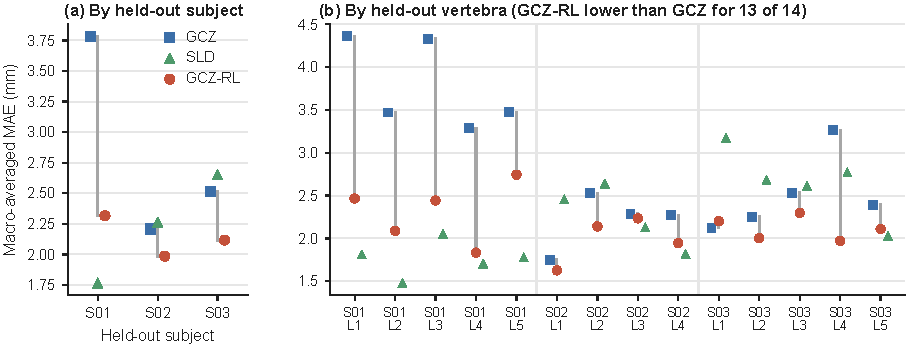
\includegraphics[width=\textwidth]{fig5_patient_level.pdf}
\caption{\rev{Primary evaluation by held-out subject and by held-out vertebra (macro-averaged MAE over the classes of each unit). (a) GCZ (square) and GCZ-RL (circle) for each held-out subject, joined by a line, with the relative reduction computed from the unrounded per-case errors (values of Table~\ref{tab:loso_subject}: S01 3.784 to 2.315~mm, S02 2.208 to 1.986~mm, S03 2.512 to 2.117~mm). (b) Difference GCZ minus GCZ-RL for each of the 14 held-out lumbar vertebrae, grouped by subject; values above zero mean a lower error with GCZ-RL. GCZ-RL was lower for 13 of the 14 vertebrae; the exception is S03 L1 (2.124 against 2.200~mm, open circle). The vertebrae are nested within three subjects and are not independent patients. SLD is compared in Tables~\ref{tab:loso_ligament}, \ref{tab:loso_subject}, and~\ref{tab:overall}.}}
\label{fig:patient_level}
\end{figure*}

\begin{figure*}[!t]
\centering
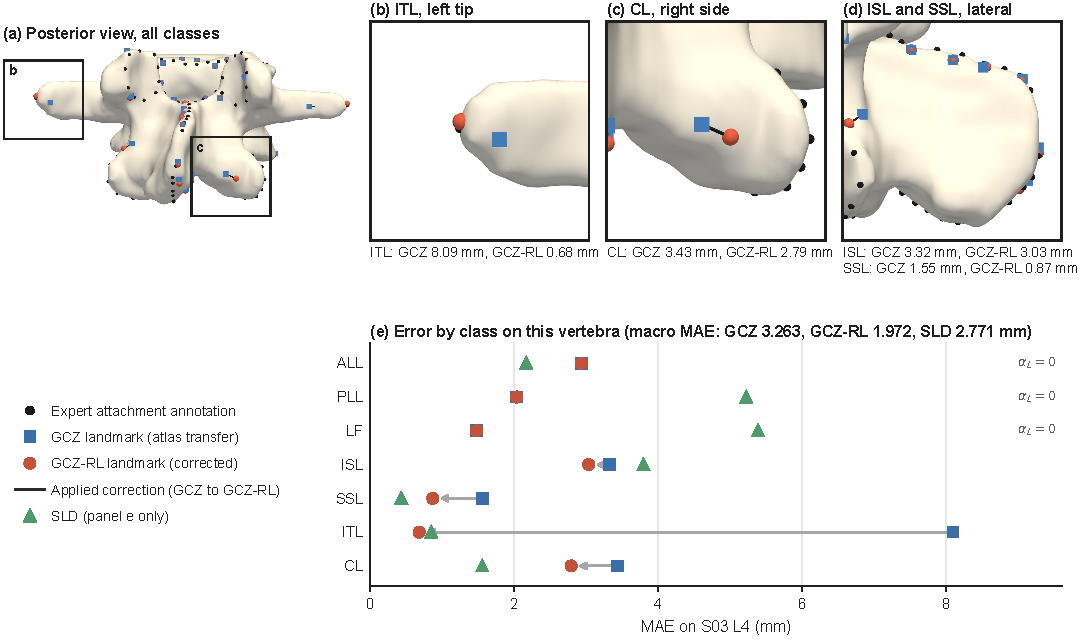
\includegraphics[width=\textwidth]{fig_qualitative_insets.pdf}
\caption{\rev{GCZ and GCZ-RL on held-out vertebra S03 L4 of the primary evaluation (subject S03, level L4; fold holding out S03; atlas S01 L1). Black spheres: expert reference annotations; blue cubes: GCZ landmarks after atlas transfer; red spheres: GCZ-RL landmarks; dark segments: the applied correction. All markers are the saved coordinates on the real mesh, drawn as glyphs of fixed size in millimeters, for the four classes whose correction is active in this fold. (a) Posterior view (the patient's right on the right) with thin black frames; each close-up (b--e) is exactly the part of this render inside its frame. (b) Right facet joint: the superior capsular references (CL\_S\_R, all visible in this view) and the three CL landmarks paired with them (errors 1.886 to 2.311~mm, 1.730 and 0.632~mm unchanged); the CL class error fell from 3.435 to 2.790~mm mainly through landmarks of the inferior capsule, which faces anterolaterally and is hidden in this view. (c) Spinous process with ISL (3.318 to 3.032~mm) and SSL (1.554 to 0.867~mm). (d, e) Right and left transverse processes in full: the GCZ landmarks lie on the posterior surface of the processes, inside the wide GCZ selection region and outside the projection region, and GCZ-RL places them at the tips (right 11.508 to 0.590~mm, left 4.682 to 0.765~mm; ITL class error 8.095 to 0.678~mm). (f) Class error of GCZ, GCZ-RL, and SLD on this vertebra (mean of the Hungarian-matched pairs, as in Table~\ref{tab:loso_ligament}); arrows run from GCZ to GCZ-RL. For ALL, PLL, and LF the inner validation of this fold selected $\alpha_L=0$, so GCZ and GCZ-RL coincide; their attachment margins are shown in Fig.~\ref{fig:regions_footprints}. Macro-averaged errors on this vertebra: 3.263~mm (GCZ), 1.972~mm (GCZ-RL), and 2.771~mm (SLD), against cohort means of 2.879, 2.150, and 2.224~mm. The vertebra shows the correction clearly but is not a typical case: its improvement ranks fifth of the 14 held-out vertebrae. Every landmark, its matched reference, its error, and its visibility are listed in \texttt{fig7\_landmark\_verification\_S03\_L4.csv} of the code release; the three methods for all seven classes in three views are in Supplementary Fig.~S7.}}
\label{fig:qualitative_loso}
\end{figure*}

\begin{table*}[!t]
\centering
\revfloat
\caption{Primary evaluation: matched-pair and matching-independent metrics side by side (14 held-out lumbar vertebrae, 98 vertebra--class cases). Difference: GCZ-RL minus the method in the row, macro-averaged MAE, with 95\% vertebra-level cluster-bootstrap interval; $p$: two-sided Wilcoxon signed-rank test over the 98 cases. P$\rightarrow$R: mean distance from each prediction to its nearest reference point. R$\rightarrow$P: mean distance from each reference point to its nearest prediction. Ref.\ ${\le}5$: reference points with a prediction within 5~mm. Paired ref.: reference points paired by Hungarian matching, which depends on the number of predictions and is not a geometric coverage measure. Best value per column in bold.}
\label{tab:overall}
\renewcommand{\arraystretch}{1.12}
\small
\resizebox{\textwidth}{!}{%
\begin{tabular}{@{}lrlrrrrrrr@{}}
\toprule
 & \multicolumn{4}{c}{\textbf{Matched pairs}} & \multicolumn{4}{c}{\textbf{Matching independent}} & \\
\cmidrule(lr){2-5}\cmidrule(lr){6-9}
\textbf{Method} & \textbf{MAE (mm)} & \textbf{Difference [95\% CI] (mm)} & \textbf{$p$} & \textbf{Pass@5 (\%)} & \textbf{P$\rightarrow$R (mm)} & \textbf{R$\rightarrow$P (mm)} & \textbf{Symmetric (mm)} & \textbf{Ref.\ ${\le}5$ (\%)} & \textbf{Paired ref.\ (\%)} \\
\midrule
\inputrows{tables/tab_overall.tex}
\bottomrule
\end{tabular}}
\end{table*}

\subsection{Component analyses}
\label{ssec:component_results}

\revstart
The three functions of the framework were examined separately on the primary evaluation, using the stored ICP geometry and the fold models of the primary run; these analyses decompose the evaluated pipeline and select nothing (Supplementary Sections~S8--S11).

\emph{Anatomy-informed candidate-region calibration.} The regions contained 90.0\% of the reference landmarks of the held-out vertebrae (Table~\ref{tab:compactness}). They did so while covering a median of 8.1--26.9\% of the vertebral surface area for the five dense classes and 0.4\% and 0.1\% for SSL and ITL, whose regions are a small patch at the spinous and transverse process tips. ALL combined the highest containment (96.7\%) with 20.3\% of the surface; PLL had the lowest containment (83.7\%) at 9.7\%. The area fractions varied little between held-out subjects (Supplementary Table~S11). Coverage and compactness are thus separate properties: a region that admitted the whole vertebra would contain every landmark and constrain nothing. Rendering the regions separately from the expert annotations and from the GCZ-RL landmarks (Fig.~\ref{fig:regions_footprints}) shows what they are: search regions that contain the attachment footprints, not segmentations of them. The expert points lie along margins, borders, and process tips, whereas the regions of ALL, PLL, and CL extend over the full superior--inferior height: the $z_n$ band of a class must contain its superior and inferior parts in every training vertebra, and these lie at different normalized heights in different vertebrae (for ALL, the inferior margin lies between $z_n=0.05$ and $0.50$), so the band spans 0.00--1.00 for ALL and CL in the fold holding out S03. The superior--inferior position of the landmarks is set by the atlas transfer, and the region constrains their antero-posterior and lateral position: none of the 280 ALL and PLL landmarks of GCZ-RL lies in the middle half between the superior and inferior body margins (Supplementary Section~S16). Taking the surface within 2.5~mm of the expert points as the footprint, the regions of the six classes other than ITL are 2.5--6.3 times larger than their footprints and contain 86--97\% of the footprint area; the ITL region consists of the most lateral vertices at the transverse process tips and is smaller than its footprint (Supplementary Section~S14).

\emph{Atlas-based geometric initialization.} The selected atlas was of the same level as the target for 7 of the 14 held-out vertebrae (Supplementary Table~S14). Same-level atlases did not give lower GCZ errors (mean per-vertebra macro MAE 3.073~mm against 2.686~mm for cross-level atlases, a comparison confounded by subject because most same-level choices concern S01), and the quick-ICP residual was not associated with the GCZ error (Spearman $\rho=0.24$, $p=0.40$; Fig.~\ref{fig:components}d). Within this residual range, a lower surface distance therefore did not indicate a better landmark transfer, which is consistent with the sensitivity of the atlas choice described in Section~\ref{ssec:implementation}: in the second computing environment, S02 L3 received an atlas with a lower residual (1.33 against 1.51~mm) but a GCZ error of 6.28 instead of 2.29~mm. GCZ-RL improved on GCZ for 13 of the 14 vertebrae, whether the atlas was of the same or a different level.

\emph{Sensitivity to the ICP seeds.} To quantify how much the results depend on the atlas selection, the complete nested procedure was re-run ten times with the ICP alignments recomputed from scratch and the random seeds of the ICP point sampling shifted; the subjects and folds, calibration, regressors, hyperparameters, model-selection grid, and evaluation were unchanged (Supplementary Section~S13). These runs are a computational sensitivity analysis on the same three subjects, not additional subjects or an external validation. Between 2 and 4 of the 14 held-out vertebrae changed atlas in each run. GCZ-RL improved on GCZ in all ten runs, by 22.8--33.4\% (mean 26.9\%), and for every held-out subject in every run (30 of 30 subject--run comparisons; Fig.~\ref{fig:icp_seeds}). The absolute error depended on the atlas selection: GCZ-RL reached 2.10--2.92~mm (mean $2.36\pm0.24$~mm) and GCZ 2.84--3.89~mm (mean $3.23\pm0.31$~mm). The reported values, 2.150 and 2.879~mm, are those of the stored alignments and lie in the lower part of these ranges.

\emph{Constrained residual refinement.} Table~\ref{tab:ablation} adds the elements of the refinement one at a time; the complete configuration reproduces the reported GCZ-RL predictions exactly. The two elements of the refinement, the learned correction and the projection onto the calibrated regions (Eqs.~\eqref{eq:corrected_point} and~\eqref{eq:projection}), act together. The predicted residual without projection lowered the macro-averaged MAE from 2.879 to 2.698~mm but left every corrected point off the surface (mean distance 0.57~mm), which is why the method projects it back. The correction bound was not reached by any held-out point (none of the 742 predicted corrections exceeded $\tau_L$); it acts as a safeguard against extrapolation and did not alter any prediction in this cohort. Projection of the corrected points gave 2.132~mm and placed every output on the vertebral surface and 740 of the 742 outputs on a vertex of the projection region; the other two are the ITL points of S01 L5 and S02 L4, which keep their GCZ position because the region has no vertex on their side (Section~\ref{ssec:loso}).

Projection alone, without the learned residual, is the strongest geometry-only configuration (2.310~mm). It changes only ITL, from 6.262 to 2.279~mm, because the GCZ selection step of ITL used its widest fallback band in all 14 vertebrae (Supplementary Table~S4), whereas the projection region is a small patch at the transverse process tips (Table~\ref{tab:compactness}); the GCZ points of the other classes already lie in their projection regions. The learned correction improved on this strongest geometry-only configuration in each of the three held-out subjects (from 2.563 to 2.315~mm for S01, 2.042 to 1.986~mm for S02, and 2.273 to 2.117~mm for S03), and GCZ-RL reached 2.150~mm overall (difference $-0.160$~mm, 95\% cluster-bootstrap interval $-0.234$ to $-0.085$~mm; lower error in 45 and higher in 15 of the 98 cases, Wilcoxon $p<0.001$). It lowered the ITL error further to 1.796~mm and, over the six other classes, reduced the macro-averaged error from 2.316 to 2.209~mm ($p<0.001$ over 84 cases), again with a reduction for every held-out subject. As in Section~\ref{ssec:correspondence}, the paired tests and intervals describe the consistency of the differences across the vertebra--class cases of this cohort; the improvement in each of the three independent subjects is the more direct evidence. Applying the full correction to every class ($\alpha_L=1$) would have given 2.132~mm. This is a comparison made after the held-out subjects had been evaluated: choosing $\alpha_L$ on the basis of held-out performance would remove the independence of the evaluation, so 2.150~mm remains the result of the pre-specified method, whose blend weights were chosen by the nested inner validation. That this choice scored slightly worse than the uniform weight on the held-out subjects also shows that the selection did not favor the reported result. The side constraint is required for ITL: when the nested procedure was re-run without it, the two ITL points of 2 of the 14 vertebrae were projected onto the same transverse process, an anatomically invalid output that the constraint excludes (Supplementary Section~S8).

The learned corrections were directionally consistent with the true residuals and conservative in magnitude (Supplementary Section~S10). Over all held-out GCZ points, the predicted residual pointed within 90$^\circ$ of the true residual for 67.1\% of points, with a median length of 47\% of the true residual, which is the behavior expected of an averaging ensemble trained on few subjects. Grouped permutation importance showed that every feature group contributed, with an ordering that differed between folds (Fig.~\ref{fig:components}c); by impurity, the relation of the point to its candidate region (37.7\% of the total) and its normalized position (25.5\%) were used most, followed by the offset from the class prior (19.3\%). These importances describe what the fitted models use and do not by themselves establish an anatomical mechanism.
\revend

\begin{table*}[!t]
\centering
\revfloat
\caption{Component ablation of the primary evaluation (14 held-out vertebrae, 98 vertebra--class cases). Each row adds one element to the GCZ prediction, using the stored ICP geometry and the fold models of the primary run. $p$: Wilcoxon signed-rank test against GCZ over the 98 cases. Admissible: outputs that are vertices of the projection region of their class; in the complete configuration, the two exceptions are ITL points that keep their GCZ position under the side constraint (Section~\ref{ssec:loso}). Surface: mean distance of the outputs to the vertebral surface. The row with $\alpha_L=1$ is a comparison made after the held-out evaluation and was not used to choose the method. The complete configuration reproduces the reported GCZ-RL predictions exactly and improves on the strongest geometry-only configuration, GCZ with projection, in each held-out subject (difference $-0.160$~mm, 95\% interval $-0.234$ to $-0.085$~mm).}
\label{tab:ablation}
\renewcommand{\arraystretch}{1.12}
\small
\resizebox{\textwidth}{!}{%
\begin{tabular}{@{}lrrrrrrrr@{}}
\toprule
\textbf{Configuration} & \textbf{MAE (mm)} & \textbf{$p$ vs.\ GCZ} & \textbf{Pass@5 (\%)} & \textbf{R$\rightarrow$P (mm)} & \textbf{Ref.\ ${\le}5$ (\%)} & \textbf{ITL MAE (mm)} & \textbf{Admissible (\%)} & \textbf{Surface (mm)} \\
\midrule
\inputrows{tables/tab_ablation.tex}
\bottomrule
\end{tabular}}
\end{table*}

\begin{table}[!t]
\centering
\revfloat
\caption{Candidate-region coverage and compactness on the held-out vertebrae of the primary evaluation (14 per class). Inside: reference landmarks whose nearest vertex lies in the region of their class (Supplementary Table~S4). Vertices: median number of region vertices (meshes have a median of 33{,}445). Vertex and area fractions: median (interquartile range) share of the mesh vertices and of the vertebral surface area that belongs to the projection region; area uses triangle areas.}
\label{tab:compactness}
\renewcommand{\arraystretch}{1.12}
\scriptsize
\resizebox{\columnwidth}{!}{%
\begin{tabular}{@{}lrrrll@{}}
\toprule
\textbf{Class} & \textbf{Ref.} & \textbf{Inside (\%)} & \textbf{Vertices} & \textbf{Vertex fraction (\%)} & \textbf{Area fraction (\%)} \\
\midrule
\inputrows{tables/tab_compactness.tex}
\bottomrule
\end{tabular}}
\end{table}

\begin{figure*}[!t]
\centering
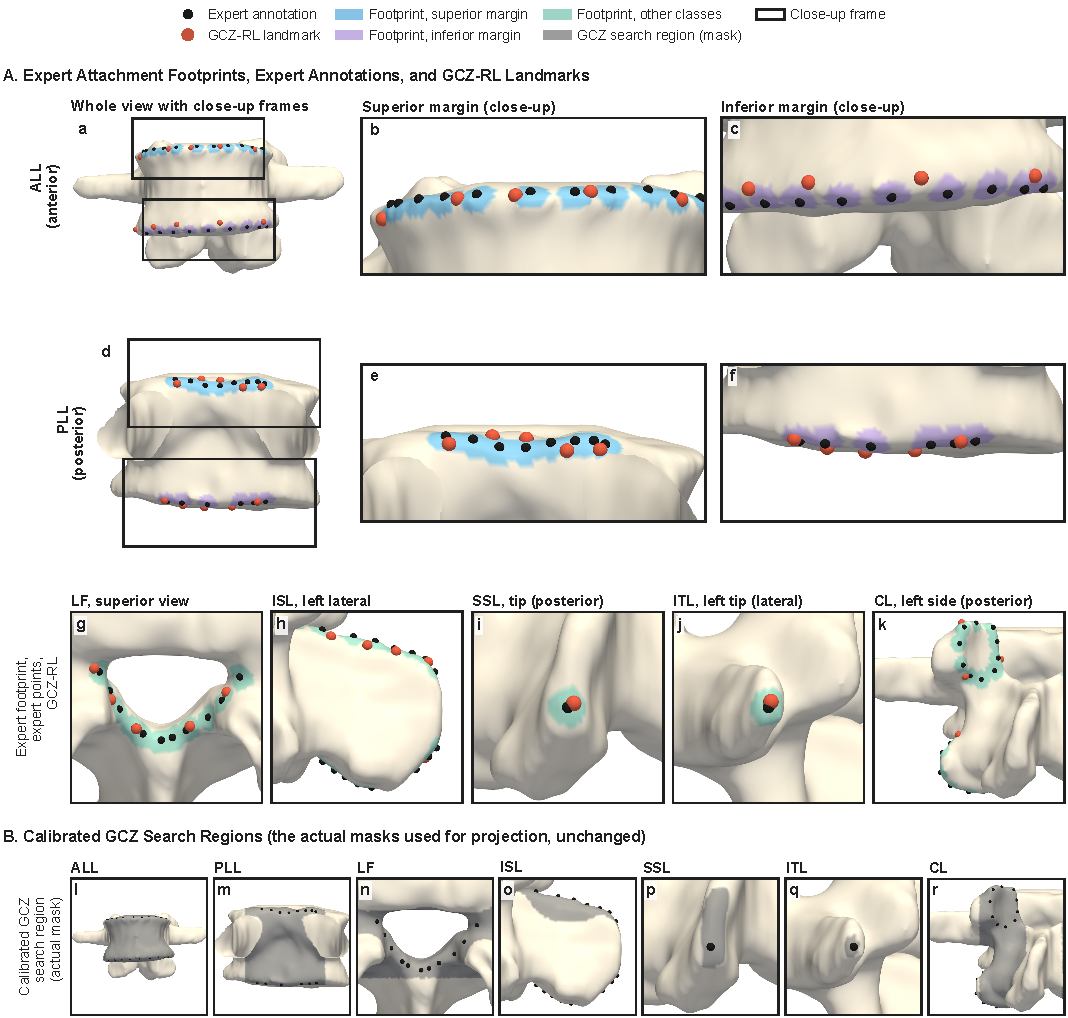
\includegraphics[width=\textwidth]{fig_regions_margins.pdf}
\caption{\rev{Attachment anatomy and calibrated search regions on held-out vertebra S03 L4 (regions calibrated on the training subjects S01 and S02). Part A: expert attachment footprints, expert annotations (black), and GCZ-RL landmarks (red). A footprint is the mesh surface within 2.5~mm of the expert points of a class (the definition of Supplementary Section~S14); it is derived from the annotations, follows the bony contour, and is not a model output. (a--c) ALL in the anterior view and (d--f) PLL in the posterior view of the vertebral body (posterior arch removed for display): superior (blue) and inferior (lavender) margin footprints on the natural bone color, with thin black frames marking the close-ups of the superior (b, e) and inferior (c, f) margins, cropped from the same render at one scale (46 by 21~mm). (g--k) LF, ISL, SSL, ITL, and CL with their footprints (green), one camera per class; SSL and ITL are viewed end-on at the spinous and left transverse process tips. Part B, Calibrated GCZ Search Regions: (l--r) the masks used for projection (gray), drawn exactly as computed with the expert points and not narrowed. For ALL, PLL, and CL they cover the surface between the attachment margins, because one band must contain the margins of all training vertebrae (Supplementary Section~S16); every GCZ-RL landmark is a vertex of its search region, and the landmarks lie on the attachment margins.}}
\label{fig:regions_footprints}
\end{figure*}

\begin{figure*}[!t]
\centering
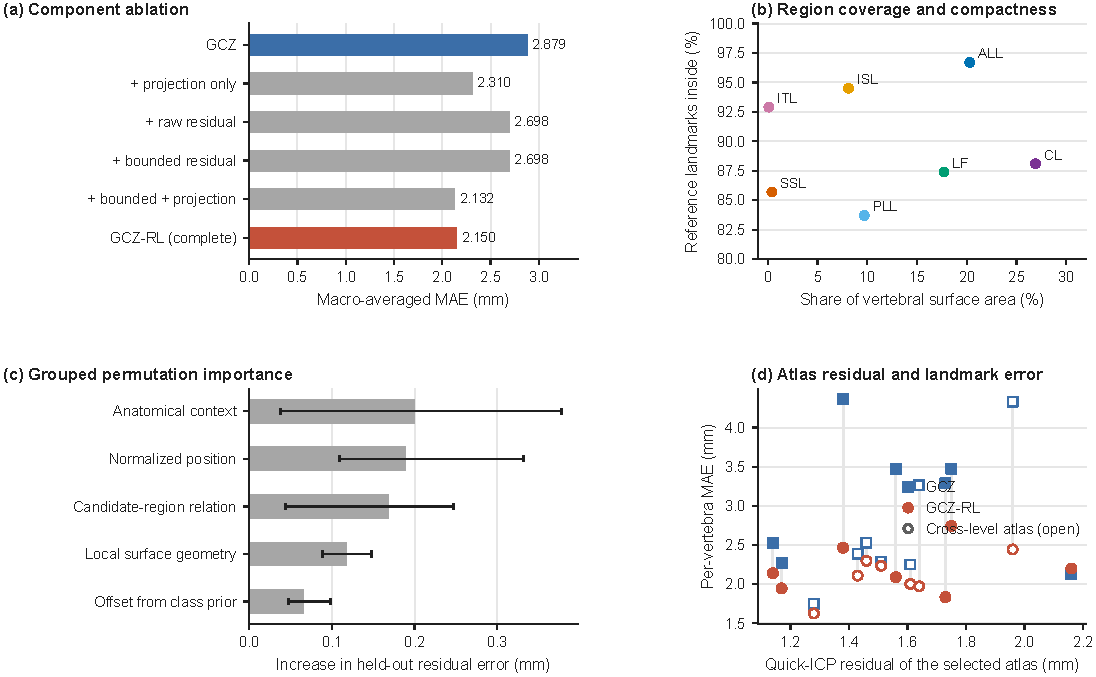
\includegraphics[width=0.95\textwidth]{fig7_components.pdf}
\caption{\rev{Component analyses of the primary evaluation. (a) Macro-averaged MAE of the six configurations of Table~\ref{tab:ablation} in methodological order, from GCZ to the complete GCZ-RL; values to three decimals at the right; the horizontal axis starts at 1.9~mm. The configuration with $\alpha_L=1$ is an ablation; the complete GCZ-RL uses the blend weights $\alpha_L$ selected by the inner validation of each fold. (b) Containment of the reference landmarks against the share of the vertebral surface covered by the projection region, one point per class (Table~\ref{tab:compactness}); the vertical axis starts at 80\%. (c) Grouped permutation importance of the residual regressors: increase in the held-out residual-prediction error when one feature group is permuted; short vertical ticks, the three folds; diamond, their mean; gray line, their range. (d) Quick-ICP residual of the selected atlas against the per-vertebra macro MAE of GCZ (squares) and GCZ-RL (circles); filled markers, same-level atlas; open markers, cross-level atlas; gray segments connect the two methods on each vertebra; thin white marker edges keep coincident values visible, and no value is moved.}}
\label{fig:components}
\end{figure*}

\begin{figure*}[!t]
\centering
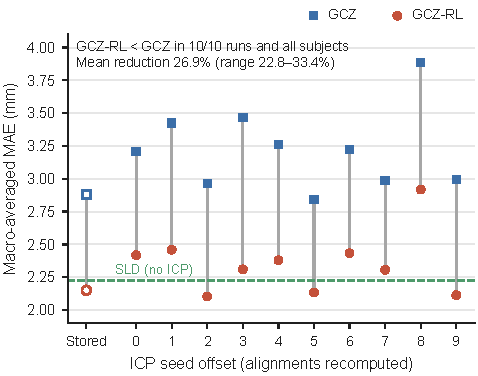
\includegraphics[width=4.9in]{fig8_icp_seeds.pdf}
\caption{\rev{Sensitivity of the primary evaluation to the ICP atlas selection. Macro-averaged MAE of GCZ (squares) and GCZ-RL (circles), joined for each run. Left of the divider: the stored alignments of the reported results (open markers; GCZ 2.879~mm, GCZ-RL 2.150~mm). Right: ten runs in which all ICP alignments were recomputed with shifted sampling seeds and everything else was unchanged (filled markers; GCZ-RL 2.10--2.92~mm, mean 2.357~mm; GCZ mean 3.226~mm). GCZ-RL improved on GCZ in every run, by 22.8--33.4\% (mean 26.9\%), and for every held-out subject in every run. Dashed line: SLD (2.224~mm), which does not use ICP. The absolute error, and with it the ordering relative to SLD, depends on the selected atlases. This is a computational sensitivity analysis on the same three subjects, not ten independent cohorts (Supplementary Section~S13).}}
\label{fig:icp_seeds}
\end{figure*}

\subsection{Supplementary development analysis: vertebra-wise split}

Table~\ref{tab:literature} and Fig.~\ref{fig:literature_chart} characterize development behavior across cervical, thoracic, and lumbar levels. Residual refinement reduced the macro-averaged mean Euclidean error of the GCZ baseline from 3.708 to 2.946~mm and raised Pass@5 from 79.8\% to 88.1\%, with improvements in both metrics for all seven classes; the largest gains were for LF (4.110 to 2.933~mm) and CL (5.437 to 3.426~mm), the classes for which rigid transfer alone performed worst. The GCZ column of Table~\ref{tab:literature} is the geometry-only configuration as originally evaluated on the STL surfaces; GCZ-RL corrects a second GCZ run on the equivalent VTK surfaces of the same vertebrae, with different random seeds and without the last zone fallback, whose macro-averaged error is 3.704~mm and Pass@5 80.8\%. Relative to the points it actually corrects, GCZ-RL lowered the error significantly over the 189 scored vertebra--class cases (Wilcoxon $p<0.001$). These numbers are not an independent test, because the model configuration was influenced by the held-out results. The SLD values in Table~\ref{tab:literature} are included as descriptive context for the historical development run, which used a different surface-processing configuration and coordinate frame (Section~\ref{ssec:sld_evaluation}). Comparative interpretation of GCZ-RL and SLD is based on the common-frame primary patient-level evaluation in Table~\ref{tab:loso_ligament}.

\begin{table*}[!t]
\centering
\caption{Supplementary vertebra-wise development analysis (20 calibration and 37 held-out vertebrae; 27 held-out VerSe vertebrae scored). GCZ and GCZ-RL values quantify residual-refinement behavior in the development split. SLD values originate from the earlier adapted processing run and are included for descriptive context only; the primary common-frame comparison is provided in Table~\ref{tab:loso_ligament}. MAE is macro-averaged over classes and vertebra-level mean distances; Pass@5 pools matched pairs within class. Best value per row and metric in bold.}
\label{tab:literature}
\renewcommand{\arraystretch}{1.12}
\scriptsize
\resizebox{\textwidth}{!}{%
\begin{tabular}{@{}lrrrrrr@{}}
\toprule
\textbf{Ligament} &
\textbf{Original GCZ MAE} &
\textbf{Original GCZ Pass@5} &
\textbf{GCZ-RL MAE} &
\textbf{GCZ-RL Pass@5} &
\textbf{SLD MAE} &
\textbf{SLD Pass@5} \\
\midrule
ALL & 3.050 & 86.7\% & \textbf{2.708} & 88.1\% & 2.750 & \textbf{90.4\%} \\
PLL & 2.329 & 92.6\% & \textbf{2.164} & \textbf{94.4\%} & 2.246 & 91.8\% \\
LF  & 4.110 & 67.0\% & \textbf{2.933} & \textbf{88.5\%} & 4.814 & 60.9\% \\
ISL & 2.495 & 91.2\% & \textbf{2.277} & \textbf{94.6\%} & 4.560 & 69.5\% \\
SSL & 2.921 & 85.2\% & 2.681 & 88.9\% & \textbf{1.739} & \textbf{100.0\%} \\
ITL & 5.614 & 72.2\% & 4.434 & \textbf{81.5\%} & \textbf{3.485} & 76.7\% \\
CL  & 5.437 & 63.7\% & 3.426 & 80.7\% & \textbf{1.630} & \textbf{99.0\%} \\
\midrule
\textbf{Mean} & 3.708 & 79.8\% & \textbf{2.946} & \textbf{88.1\%} & 3.032 & 84.0\% \\
\bottomrule
\end{tabular}}
\end{table*}

\begin{figure*}[!t]
\centering
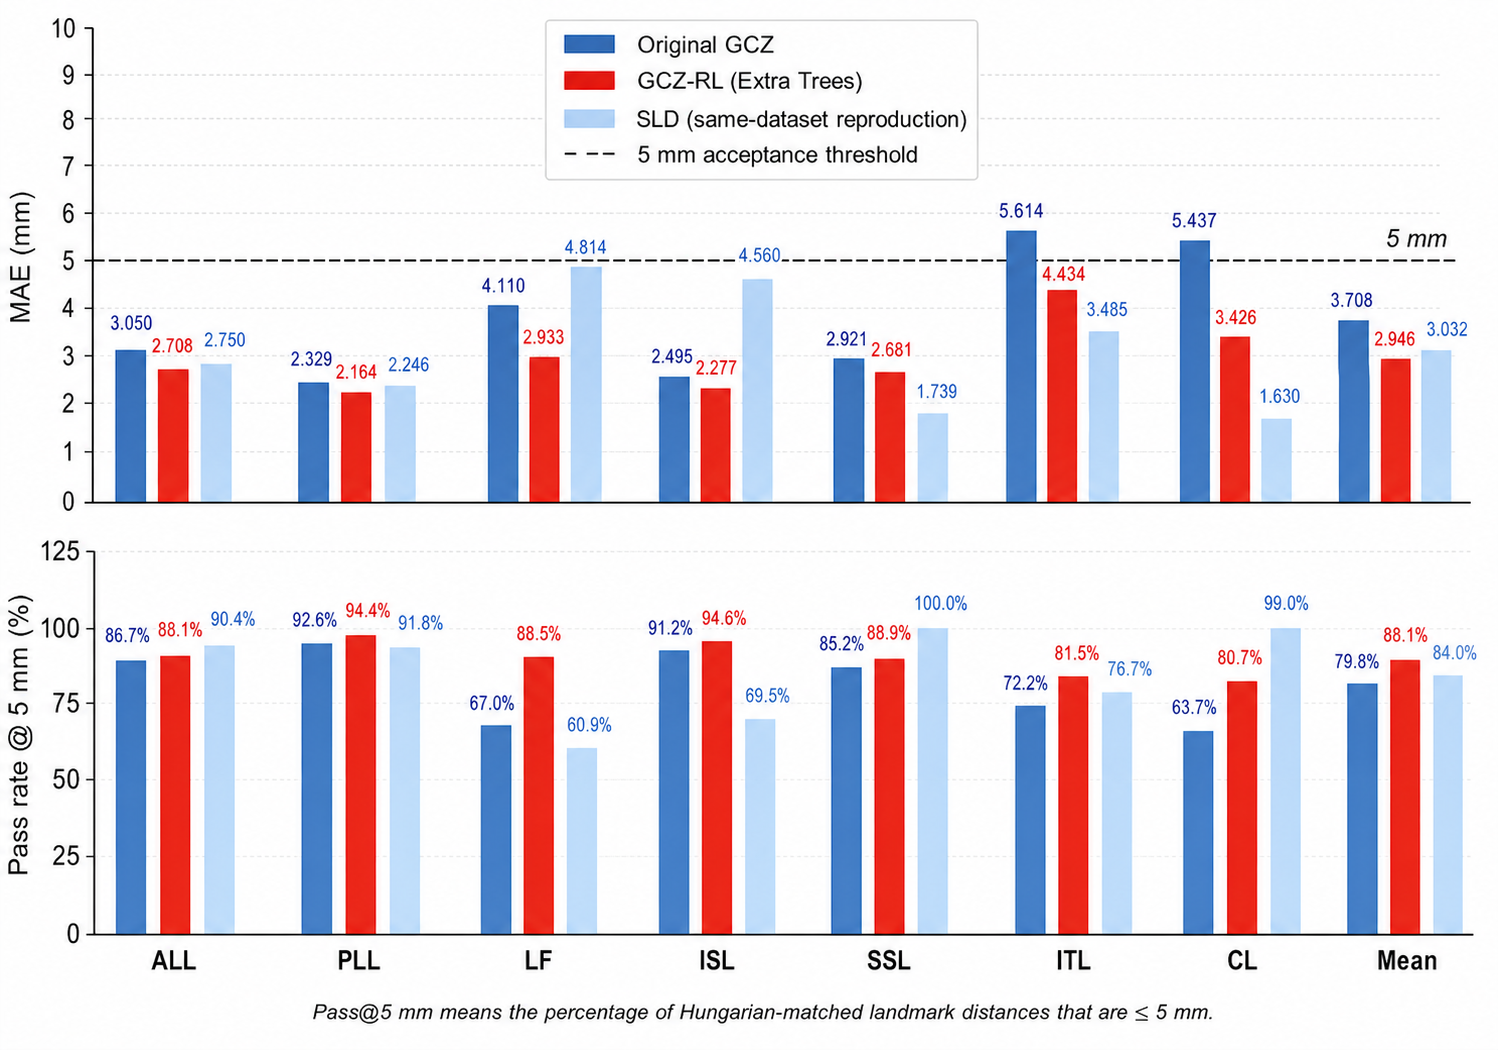
\includegraphics[width=0.8\textwidth]{fig_literature_comparison_clean2.png}
\caption{Supplementary development analysis (values of Table~\ref{tab:literature}): per-ligament mean Euclidean error (top) and Pass@5 (bottom) for the original GCZ configuration and GCZ-RL, with SLD values shown for descriptive context only. The GCZ-RL configuration was partly chosen after held-out outputs had been inspected, and this SLD run used different preprocessing and a mismatched coordinate frame; the SLD values are not used for comparative ranking.}
\label{fig:literature_chart}
\end{figure*}

\subsection{Effect of the correspondence rule}

One-to-one Hungarian matching minimizes the total distance but can pair anatomically non-corresponding points, such as left--right swaps and superior--inferior inversions. A diagnostic analysis on the nine held-out lumbar vertebrae of the development analysis (Supplementary Section~S6) found that anatomy-constrained matching rules removed many long-range pairs (58 instead of 119 errors above 10~mm) at the cost of leaving about 7\% more reference landmarks unpaired. That analysis characterizes the matching rule only; the method comparison of this paper applies the same one-to-one Hungarian matching to all methods.

\subsection{Summary of the comparison}

Across the three-subject primary evaluation, the consistent finding is that \rev{the constrained refinement, bounded residual correction with projection onto the calibrated regions,} reduces the error of the geometry-only GCZ baseline, for every held-out subject and on both matched-pair and matching-independent metrics\rev{, and the learned correction improves on the strongest geometry-only configuration for each held-out subject}. GCZ-RL and the tested SLD implementation reached similar aggregate errors (2.150 and 2.224~mm, difference not significant) with different class-specific strengths, so the two approaches are best described as performing comparably; which one is ahead depends on the class and, for matching-independent metrics, on the direction of measurement\rev{, and, across recomputations of the ICP alignments, on the atlas selection, whereas the improvement over GCZ held in every recomputation}. The development analysis showed the same direction of improvement over the geometry-only baseline across cervical, thoracic, and lumbar levels. Together, these results support the combination of geometry-calibrated anatomical constraints with constrained residual learning as an effective strategy for spinal ligament landmark localization from small annotated datasets; confirming its generalization requires larger, multi-institutional cohorts.

% =====================================================================
\section{Discussion}
\label{sec:discussion}

GCZ-RL demonstrates how calibration-derived anatomical search spaces and constrained residual learning can be combined for sparse ligament landmark localization on vertebral meshes. The framework separates global surface alignment from local shape-dependent refinement: atlas transfer provides an interpretable initialization, while a bounded regressor corrects residual displacements \rev{that are projected back onto the calibrated candidate regions, with a side-preserving fallback for bilateral landmarks}. In the primary leave-one-subject-out analysis, the error reduction relative to geometry-only GCZ was observed for each held-out subject. The supplementary vertebra-wise development analysis showed the same direction of improvement over GCZ across seven ligament classes. Together, these results highlight the value of constraining the learning task rather than directly regressing unconstrained landmark coordinates from limited annotations.

Comparison with the evaluated SLD implementation shows that the two approaches have different class-dependent strengths. SLD uses distinctive surface morphology through predefined anatomical rules, whereas GCZ-RL adapts candidate regions and refinement to training annotations. This distinction is especially relevant for ligaments such as PLL and LF, for which GCZ-RL produced lower localization errors in the primary evaluation. The methodological contribution is therefore not a claim of universal superiority over SLD, but a complementary strategy that combines explicit geometry, local learning, and surface-consistent prediction.

The SLD errors measured here are higher than the 0.7~mm reported by \citet{blomenkamp2026sld} on their annotations. Under their closest-point protocol, which measures each prediction against the nearest reference point, the SLD implementation evaluated here reached 1.787~mm on the 14 lumbar vertebrae. Three factors may contribute to the remaining difference: the cross-section approximation of the VMTK centerline, differences between the vertebrae evaluated in the two studies, and the remeshing and snapping steps of the standalone pipeline. A comparison with the original 3D Slicer implementation, ideally in collaboration with its authors, would establish how much of the gap is due to the reimplementation; until then, the SLD numbers of this paper should be read as those of the evaluated implementation.

\revstart
The primary results are also supported by matching-independent measurements that assess both directions of point-set proximity. Reference-to-prediction closest-point error was 3.297~mm for GCZ-RL versus 4.089~mm for the evaluated SLD implementation; reference coverage within 5~mm was 78.4\% for GCZ-RL, 77.6\% for SLD, and 72.1\% for GCZ (Table~\ref{tab:overall}). These complementary measurements assess the spatial representation of the annotated footprints beyond the one-to-one matched pairs; in the opposite direction, from each prediction to its nearest reference point, SLD was closer (1.787 against 2.140~mm).
\revend

Two design elements were essential. First, the evaluation must make its pairing rule explicit: with dense reference footprints and ten predictions per class, one-to-one matching scores only the paired part of each footprint, so we report coverage and matching-independent metrics alongside MAE and Pass@5. Second, constraints on the output matter: \rev{projection keeps corrected landmarks on the admissible surface region, with a side-preserving fallback when required, and all final predictions remain on the vertebral surface. For the bilateral lateral classes,} a side constraint was required to prevent both points of a pair from collapsing onto one transverse process. \rev{The component analysis confirms this design. The learned correction and the projection onto the calibrated regions act together: each corrected landmark is a learned refinement constrained to the admissible surface region, with the side-preserving fallback when required, the complete method improves on the strongest geometry-only configuration for each held-out subject, and the side constraint excludes anatomically invalid ITL pairs. The calibrated regions are therefore not only a safeguard but an active part of the localization, which is the central principle of GCZ-RL: anatomy defines the admissible solution space, and learning refines the position within it. The improvement over GCZ also held for every held-out subject when the ICP alignments were recomputed with ten different seeds, although the absolute accuracy varied with the selected atlases; a more robust atlas initialization, for example by pre-alignment or multi-start ICP, is the most direct route to higher and more stable absolute accuracy.}

A practical advantage is interpretability. Each prediction follows a visible chain of zone assignment, atlas transfer, selection, correction, and projection, so a large error can be traced to a zone that excludes the expert landmark, a poor atlas match, a clipped correction, or annotation variability. The containment analysis makes one such limit explicit: about one in ten reference landmarks lies outside the zone of its class, most often at L5 and for PLL, and no correction can reach these points.

\revstart
\emph{Relation to finite element modeling.} The localized landmarks are geometric inputs for subject-specific spine models, in which ligaments are commonly represented by tension-only elements between their attachment sites~\citep{dreischarf2014}. A finite element assessment of predicted against reference attachment sites would additionally require ligament definitions that connect the landmarks of adjacent vertebrae, material properties, boundary and loading conditions, and a model validated against experimental data, whose outputs, such as range of motion or ligament strain and force, could then be compared between the two sets of attachments. The present study evaluates the localization stage only and makes no claim about mechanical outcomes. A focused follow-up, in which the same validated motion-segment model is run once with reference and once with predicted attachments, would quantify how localization errors of the size measured here propagate to ligament lengths and forces. It is a separate, downstream assessment rather than a prerequisite for measuring localization accuracy.

\emph{Annotated data and external validation.} Public expert annotations of ligament attachments are scarce, and this is the setting for which GCZ-RL was designed; the primary evaluation therefore rests on three independent subjects. Additional annotated cohorts, ideally with documented annotation protocols and inter-observer reliability, would allow an external validation that leaves the present held-out evaluation untouched, once their compatibility in ligament definitions, vertebral levels, and mesh representation has been established.
\revend

\subsection{Limitations}

The present study evaluates localization against a single set of expert annotations and reports subject-level leave-one-out results on 14 lumbar vertebrae from three subjects. \rev{The source publications of these annotations do not report the number or qualifications of the annotators or an inter-observer reliability analysis, so annotation variability is contained in all reported errors and cannot be quantified here.} Accordingly, the results characterize performance within this annotated cohort rather than population-level clinical accuracy, and the paired statistics describe consistency within the cohort rather than generalization. The additional vertebra-wise analysis is presented as development evidence. The anatomy-based lateral projection constraint was introduced after inspection of an earlier evaluation output and is disclosed as a design refinement\rev{; the component analysis shows that it is required for anatomically valid ITL pairs (Section~\ref{ssec:component_results})}. The SLD comparison uses the released implementation with a cross-section-centroid approximation of its centerline component, and its errors are higher than those published for SLD. The ICP-based atlas selection is sensitive to small numerical differences\rev{ and to the random sampling of ICP: across ten recomputations of the alignments with different seeds, 2--4 of the 14 held-out vertebrae changed atlas, and GCZ-RL reached 2.10--2.92~mm (mean 2.36~mm) instead of the reported 2.150~mm, with the improvement over GCZ preserved in every run but not the ordering relative to SLD (Supplementary Sections~S5 and S13)}. GCZ and GCZ-RL output at most ten landmarks per class, so they describe each attachment footprint by a sparse subset rather than a complete curve. Candidate-region membership confirms adherence to the calibrated geometric search rules, while the accuracy of the resulting landmarks is assessed separately against the reference annotations. Effects on downstream biomechanical simulation are beyond the present localization evaluation.

% =====================================================================
\section{Conclusion}
\label{sec:conclusion}

We presented GCZ-RL, a framework for sparse spinal ligament landmark \rev{localization} that couples annotation-calibrated anatomical search spaces with rigid atlas transfer and bounded residual refinement. In leave-one-subject-out evaluation on 14 lumbar vertebrae from three subjects, GCZ-RL reduced macro-averaged mean Euclidean localization error from 2.879 to 2.150~mm relative to geometry-only GCZ and improved the 5-mm pass rate from 86.0\% to 92.7\%, with consistent gains across held-out subjects\rev{, which were preserved for every subject when the ICP alignments were recomputed with ten different seeds}. \rev{Component analyses showed that the calibrated regions contain 90\% of the reference landmarks while covering a small part of the vertebral surface, that the learned correction and the projection onto these regions act together, and that the complete method improves on the strongest geometry-only configuration for each held-out subject.} The evaluated SLD implementation achieved comparable aggregate performance (2.224~mm), with distinct strengths across ligament classes. The supplementary vertebra-wise development analysis likewise showed improvement over the geometry-only baseline. These findings support geometry-calibrated residual learning as an interpretable, surface-consistent approach to spinal ligament landmark localization in small annotated datasets. \rev{The localized landmarks are geometric inputs for subject-specific biomechanical models; how their errors propagate to mechanical outcomes remains to be assessed in a validated model.}

\section*{CRediT authorship contribution statement}
%% Roles must use the CRediT taxonomy; every author should confirm their own roles.
\textbf{Mohsen Ahmadi:} Conceptualization, Methodology, Software, Validation, Formal analysis, Investigation, Data curation, Writing -- original draft, Visualization.
\textbf{Maohua Lin:} Conceptualization, Supervision, Writing -- review \& editing, Funding acquisition.
\textbf{Yufei Tang:} Supervision, Methodology, Writing -- review \& editing, Funding acquisition.
\textbf{Frank D. Vrionis:} Writing -- review \& editing. %% previous draft: "Clinical guidance", which is not a CRediT role (consider Validation or Resources)

\section*{Declaration of competing interest}
The authors declare that they have no known competing financial interests or personal relationships that could have appeared to influence the work reported in this paper.

\section*{Data and code availability}
\textit{Data.} The vertebral surface meshes and ligament annotations analyzed in this study are derived from public datasets: VerSe~\citep{sekuboyina2021} for the CT data of subjects S01--S03, and the ligament-landmark datasets released with SLD~\citep{blomenkamp2026sld,spinetoolkit2026} for the annotations of all subjects and the cervical vertebrae of S04--S05. They can be obtained from the original sources under their respective terms. The vertebra-level split, the mapping between subject codes and source identifiers, and SHA-256 checksums of every input file are released with the code.

\textit{Code, models, and results.} The code, trained models, and results are available at \url{https://github.com/ahmadi-lab/GCZ_RL_Spinal_Ligament_Landmarks} and will be archived with a DOI upon publication~\citep{gczrl2026code}. The release contains (i) the Python implementation of GCZ, GCZ-RL, and the evaluation, including Hungarian matching and all metrics; (ii) the wrapper that runs the released SLD implementation with the coordinate conversion; (iii) the scripts that regenerate every table and figure of this paper, together with the stored ICP alignment results that make the reported values exactly reproducible; (iv) the trained Extra Trees models of the development analysis and of each patient-level fold; (v) the predicted landmark coordinates of all methods and the per-vertebra metrics; and (vi) the data-leakage test. The source meshes and annotations are not redistributed; a script retrieves them from their original sources and verifies them against the checksums.

\section*{Acknowledgments}
This research was supported by the National Institute of Biomedical Imaging and Bioengineering of the National Institutes of Health under Award Number R01EB025819 and by the National Science Foundation under Award 2205205. The content is solely the responsibility of the authors and does not necessarily represent the official views of the National Institutes of Health or the National Science Foundation.

\bibliographystyle{elsarticle-harv}
\bibliography{references}

\end{document}
